%clase del documento
\documentclass[pregrado]{tesis-usb}

% paquetes
\usepackage[utf8]{inputenc}
\usepackage{verbatim}
\usepackage{acronym}
\usepackage{amsmath}
\usepackage{amsfonts}
\usepackage{amssymb}
\usepackage{wallpaper}
\usepackage{dirtytalk}
\usepackage{xcolor}
\usepackage{booktabs}
\usepackage[T1]{fontenc}
\usepackage{newtxtext, newtxmath}
\usepackage{url}
\usepackage{ragged2e}
\usepackage{etoolbox}
\usepackage{titlesec}
\usepackage[spanish]{babel}
\usepackage{listings}
\usepackage{setspace}
\usepackage{xparse}
\usepackage{csquotes}
\usepackage{setspace}
\usepackage[labelfont=bf]{caption}

% configuración de referencias
\usepackage[backend=biber,style=apa]{biblatex}
\DeclareLanguageMapping{spanish}{spanish-apa} % configuración del lenguaje
\addbibresource{referencias.bib} % utilizar archivo referencias.bib para la bibliografía 

\newcommand{\Csh}{C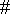
\includegraphics{hash-symbol}}
\graphicspath{ {./images/} }

\baselinestretch
\renewcommand{\baselinestretch}{1.5} % configurar tamaño interlineado base
\geometry{{margin = 3cm, 2.5cm, 2.5cm, 2.5cm}} % configurar márgenes

% configuración de espaciado de los capítulos
\makeatletter
\patchcmd{\chapter}{\if@openright\cleardoublepage\else\clearpage\fi}{}{}{}
\makeatother

% configuración para ocultar secciones del índice
\newcounter{oldtocdepth}

\newcommand{\hidefromtoc}{%
  \setcounter{oldtocdepth}{\value{tocdepth}}%
  \addtocontents{toc}{\protect\setcounter{tocdepth}{-10}}%
}

\newcommand{\unhidefromtoc}{%
  \addtocontents{toc}{\protect\setcounter{tocdepth}{\value{oldtocdepth}}}%
}

% configurando el título del proyecto
\title{\large{APLICACIÓN DE LAS 3R DE LA ECOLOGÍA EN EL\\
ÁMBITO DOMÉSTICO PARA EL\\ 
ADECUADO MANEJO DE LOS DESECHOS SÓLIDOS EN LA\\[0.2cm]
URBANIZACIÓN GUARAGUAO DE PUERTO LA CRUZ}
}

% configurando el autor
\author{\textup{Diego Ortiz}}
\makeatletter

\let \@sverbatim \@verbatim
\def \@verbatim {\@sverbatim \verbatimplus}
{\catcode`'=13 \gdef \verbatimplus{\catcode`'=13 \chardef '=13 }} 
\makeatother

% configurando el tamaño de la sangría
\setlength{\parindent}{7ex}

% comienzo del documento
\begin{document}
    \setlength{\parskip}{1em} % espaciado entre párrafos
    
    \frontmatter % colocar números romanos
    \begin{titlepage}
\newcommand{\HRule}{\rule{\linewidth}{0.5mm}}
\begin{center}
\normalsize República Bolivariana de Venezuela\\[0.1cm] 
\normalsize Ministerio del Poder Popular para la Educación\\[0.1cm]
\normalsize Unidad Educativa Instituto Experimental\\[0.1cm] 
\normalsize Asignatura: Biología\\[0.1cm] 
\normalsize 5to año\\[0.1cm] 
\end{center}
\center 
\quad\\[0.1cm]
\begin{figure}[h]
\centering

\includegraphics[width=2cm]{title/logo.png}
\end{figure}
\quad\\[0.1cm]
\makeatletter
%\HRule \\[0.2cm]
{ \huge \bfseries \@title}\\[0.5cm]
\quad\\[0.9cm]

%\HRule \\[0.8cm]
\vspace*{1cm}
\begin{minipage}{0.4\textwidth}
\begin{flushleft} \large
\normalsize{
\textup{Tutores:}\\
\textup{Lisbeth Rodríguez \\ Yanitza Rodríguez}
}
\end{flushleft}
\end{minipage}
~
\begin{minipage}{0.4\textwidth}
\begin{flushright} \large
\normalsize{
\textup{Autores:} \\
Diego Ortiz\\
Cynthia Cataldi
}
\end{flushright}
\end{minipage}\\[3cm]
\makeatother
\mbox{}
\vfill
\normalsize Puerto La Cruz, marzo de 2022
\end{titlepage}

 % colocar portada
    \begin{center}
    \textbf{APLICACIÓN DE LAS 3R DE LA ECOLOGÍA EN EL\\
ÁMBITO DOMÉSTICO PARA EL\\ 
ADECUADO MANEJO DE LOS DESECHOS SÓLIDOS EN LA\\
URBANIZACIÓN GUARAGUAO DE PUERTO LA CRUZ}
\end{center}

\vspace*{1.5cm}

\begin{center}
    \textbf{Aprobado por:}
\end{center}

\vspace*{3cm}

\begin{figure}[h]
   \begin{minipage}{0.48\textwidth}
     \centering
     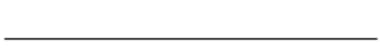
\includegraphics[width=6.cm]{Media/line.jpg}
   \end{minipage}\hfill
   \begin{minipage}{0.48\textwidth}
     \centering
     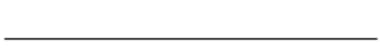
\includegraphics[width=6cm]{Media/line.jpg}
   \end{minipage}
\end{figure}

\vspace{1.5cm}

\begin{figure}[h]
    \centering
    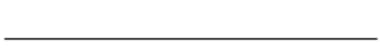
\includegraphics[width=6cm]{Media/line.jpg}
\end{figure}

\chapter*{Página de los jurados}

\newpage % colocar página de los jurados
    \hidefromtoc
\chapter*{Dedicatoria}
\unhidefromtoc

parrafo

\newpage % colocar página de la dedicatoria
    {\setlength{\parskip}{-0.5cm}
\chapter*{Agradecimientos} 

Primeramente, le agradecemos a Dios por darnos la oportunidad de trabajar en este proyecto y poder culminarlo con excelencia cumpliendo con las metas trazadas.
}

A nuestros padres, las personas que a lo largo de la vida nos apoyaron para cumplir todas nuestras metas. 

A nuestras tutoras, Lisbeth Rodríguez y Yanitza Rodríguez, por la ayuda que nos brindaron a lo largo de la elaboración de nuestro proyecto y por ser nuestras profesoras por casi todo el bachillerato, así como a todos los demás docentes que nos impartieron sus conocimientos.

Además, le damos especiales gracias a la Lic. Flor de Tepedino y el Ing. Juan Ortiz, por su gran ayuda y colaboración durante el desarrollo de la investigación.

Por último, les damos las gracias a nuestros amigos más cercanos, Oriana Cubillán, Jesús Lira, Berenice Barber, Larissa Mantilla, Valentina Figueroa y Pedro Fuentes, con quienes compartimos buenos momentos en nuestro recorrido por la Unidad Educativa Instituto Experimental.

\newpage % colocar página de los agradecimientos

    \mainmatter % regresar a la enumeración en números arábigos
    \setcounter{page}{1} % empezar el contador a partir del índice en 1
    \tableofcontents % colocar índice
    \newpage
    \listoffigures % colocar lista de figuras
    \newpage
    siguiente página del índice de figuras
    \newpage
    \listoftables
    \newpage
    \begin{center}
República Bolivariana de Venezuela\\[0.1cm] 
Ministerio del Poder Popular para la Educación\\[0.1cm]
Unidad Educativa Instituto Experimental\\[0.1cm] 
Asignatura: Biología\\[0.1cm] 
5to año\\[0.1cm] 
\end{center}

\begin{center}
    \textbf{\large{APLICACIÓN DE LAS 3R DE LA ECOLOGÍA EN EL\\
ÁMBITO DOMÉSTICO PARA EL\\ 
ADECUADO MANEJO DE LOS DESECHOS SÓLIDOS EN\\[0.2cm]
URBANIZACIÓN GUARAGUAO DE PUERTO LA CRUZ}}\\[0.1cm]
\end{center}

\vspace*{0.3cm}
\begin{flushright}
\textup{Tutores:}\\
\textup{Lisbeth Rodríguez \\ Yanitza Rodríguez}
\end{flushright}

\begin{flushright}
Autores: \\
Diego Ortiz\\
Cynthia Cataldi
\end{flushright}
\begin{flushright}
Puerto La Cruz, marzo de 2022
\end{flushright}
\vspace*{1cm}

\spacing{1}

{\setlength{\parskip}{-0.5cm}
\chapter*{Resumen}

Las 3R de la ecología son principios para fomentar el consumo responsable y el manejo adecuado de los desechos sólidos, con el fin de reducir los efectos perjudiciales en el medio ambiente causados por la contaminación. El objetivo de este trabajo fue aplicar las 3R de la ecología en el ámbito doméstico para el adecuado manejo de los desechos sólidos en la Urbanización Guaraguao de Puerto La Cruz. La investigación fue de campo y de nivel descriptivo. Se seleccionó una muestra de 22 hogares del área de estudio y se determinaron los métodos que empleaban para el manejo de la basura a través del cuestionario de preguntas cerradas. Luego, se realizó una campaña divulgativa en la que se dieron charlas junto a la distribución de folletos para la implementación de estrategias sobre las 3R de la ecología. Por último, se hizo un seguimiento para observar los métodos sugeridos que se llevaron a cabo. Se observó un cambio positivo en los hábitos de los habitantes en el manejo de los desechos sólidos; la mayoría de las estrategias propuestas fueron implementadas por la población de estudio. Se recomienda aplicar las estrategias propuestas en toda la urbanización.
}

Palabras claves: contaminación, manejo de desechos sólidos, 3R de la ecología.

\spacing{1.5}

\newpage % colocar página del resumen
    \chapter*{Introducción}

La ecología es la rama de la biología que tiene como objeto el estudio de la relación que establecen los seres vivos y el medio ambiente en el que se desarrollan, entendida como la combinación de los factores abióticos (entre los cuales se puede mencionar al clima y a la geología) y los factores bióticos (organismos que comparten el hábitat). Es un tema muy amplio que puede ser tratado desde diferentes puntos de vista como la preservación y regeneración de los recursos naturales, la protección de la vida salvaje y la reducción del nivel de contaminación generado por la humanidad.

\newpage % colocar página de la introducción
    \vspace*{6cm}
{\setlength{\parskip}{-0.5cm}
\chapter{El Problema}
}
\newpage

En este capítulo se explican de manera detallada el planteamiento del problema, el objetivo general y los específicos, y la justificación.

{\setlength{\parskip}{0cm}

\section{Planteamiento del problema}

Casi todos los países del mundo se han replanteado estilos de desarrollo diferentes con una orientación más cuidadosa con el ambiente. La medida más empleada y conocida para cumplir con esta meta es el reciclaje, el cual consiste en el proceso de recolección y transformación de materiales para convertirlos en nuevos productos, y que de otro modo serían desechados como basura.
}
Sin embargo, el concepto y la actividad del reciclaje va mucho más allá de las cuestiones técnicas y económicas, implica un esfuerzo colectivo de toda la sociedad: desde los hábitos ciudadanos en la separación de residuos para facilitar el ciclo de reciclaje, hasta las administraciones públicas que deben facilitar ese servicio. 

Además, en los países más desarrollados se suele combinar el reciclaje con otras 2 buenas prácticas para mejorar ampliamente su efectividad, formando así las 3R de la ecología: reducir y reutilizar. Reducir contribuye a la minimización de residuos producidos a diario por la sociedad, consumiendo de forma responsable. Por otra parte, reutilizar permite prolongar el tiempo de vida de los materiales, dándoles el máximo provecho posible antes de desecharlos.

En Venezuela, aún cuando se reconocen diversos problemas en materia ambiental, se cataloga a la basura como uno de los principales, debido a su incidencia en la población de cualquier estrato socioeconómico. Actualmente, no se ha inculcado en las personas hábitos de las 3R de la ecología, por lo que las mismas no aplican las normas para la clasificación de los desechos sólidos y su reducción para preservar los recursos naturales y el ambiente.

El estado Anzoátegui no es la excepción ante el desconocimiento de estas prácticas antes mencionadas dado que no se hace énfasis en una cultura de buena disposición y de poca generación de desechos y residuos, sino que por el contrario se genera en promedio por persona cerca de un kilogramo diario de desechos considerados como no reutilizables por el ciudadano común.

Específicamente, en la Urbanización Guaraguao de Puerto La Cruz, los habitantes tienen un escaso conocimiento de los métodos antes mencionados y no llevan a cabo prácticas como una buena clasificación de desperdicios para que luego puedan ser reciclados con mayor efectividad, generando un mayor desaprovechamiento de los recursos naturales y un impacto negativo al medio ambiente. 

Por todo lo anteriormente expuesto, surge la necesidad de elaborar estrategias para la aplicación de los principios de las 3R de la ecología en la Urbanización Guaraguao de Puerto La Cruz, con el propósito de incentivar el desarrollo de una cultura del reciclaje y reducir la huella ecológica de los habitantes, planteándose así la siguiente interrogante:

¿Cuáles estrategias se deben implementar para el manejo de los desechos sólidos en la Urbanización Guaraguao de Puerto La Cruz?

\newpage

{\setlength{\parskip}{0cm}
\section{Objetivo General}

Aplicar las 3R de la ecología en el ámbito doméstico para el adecuado manejo de los desechos sólidos en la Urbanización Guaraguao de Puerto La Cruz.
}

{\setlength{\parskip}{0cm}
\section{Objetivos Específicos}

Describir los beneficios que tiene el uso de las 3R de la ecología para el manejo adecuado de los desechos sólidos.
}

Establecer los métodos empleados por la población en la Urbanización Guaraguao de Puerto La Cruz para el manejo de la basura.

Realizar una campaña divulgativa sobre el manejo adecuado de los desechos sólidos para la sensibilización del uso de las 3R de la ecología en la Urbanización Guaraguao de Puerto La Cruz.

Hacer seguimiento de las estrategias propuestas para el empleo de las 3R de la ecología en la Urbanización Guaraguao de Puerto La Cruz.

\newpage

{\setlength{\parskip}{0cm}
\section{Justificación}

La acumulación de los desechos sólidos, debido al manejo inadecuado por parte de las personas, es uno de los principales problemas ambientales y de salud de la actualidad dado el constante crecimiento de la población, y de los patrones de consumo. En la Urbanización Guaraguao de Puerto La Cruz, la basura no solo crea una imagen desagradable en los espacios públicos, sino que también contamina el suelo y el aire, por lo que existe una problemática a la hora de un buen manejo de los desechos por parte de los ciudadanos. 
}

Por ello, es muy importante que los habitantes dispongan de la información pertinente para aplicar medidas que fomenten el consumo responsable y así disminuir los efectos adversos previamente mencionados. Para lograrlo, la presente investigación tiene el objetivo de aplicar los principios de las 3R de la ecología en el ámbito doméstico en la Urbanización Guaraguao de Puerto La Cruz para fomentar la cultura del manejo eficiente de los desechos sólidos.

Los principales beneficios de aplicar las 3R de la ecología en la Urbanización Guaraguao de Puerto La Cruz son: la disminución de los residuos sólidos generados por los habitantes, la mejora de las condiciones del suelo y del aire, y la sensibilización de las personas acerca de la importancia de la implementación de estos principios de la ecología, ya que constituyen una forma de iniciar el cambio antes que el medio ambiente sea contaminado del todo.
 
Además, por ser un tema de actualidad, se espera que esta investigación sirva para ampliar el conocimiento sobre las 3R de la ecología y el manejo adecuado de los desechos sólidos, y aporte algunos criterios a valorar para su aplicación, tanto en futuras investigaciones, así como de manera concreta, en la Urbanización Guaraguao de Puerto La Cruz.

\newpage
 % colocar página del capítulo 1
    \vspace*{6cm}
\chapter{Marco Teórico}
\newpage

\section{Antecedentes de la Investigación}

Durante la Cumbre del G8 (grupo de los ocho, un grupo de países con economías industrializadas del planeta) en junio de 2004, el primer ministro de Japón Koizumi Junichiro presentó la iniciativa de las 3R que busca construir una sociedad orientada hacia el reciclaje. En abril de 2005 se llevó a cabo una asamblea de ministros en la que se discutió con Estados Unidos, Alemania, Francia y otros 20 países la manera en que se puede implementar de manera internacional acciones relacionadas a las 3R. A partir de este momento, han surgido múltiples estudios acerca de la implementación de las 3R de la ecología en el marco del desarrollo sustentable y los efectos que tiene un manejo adecuado o inadecuado de los desechos sólidos.

Específicamente, en el postgrado de Muñoz P. y Leiva M. (2017) titulado \textit{Modelo municipal de reciclaje de residuos domésticos como solución ambiental}, desarrollado en la Universidad Dr. Rafael Belloso Chacín, Zulia, Venezuela, se tuvo como objetivo la formulación de un modelo que permita el manejo de los residuos domésticos y que contribuya a minimizar el impacto ambiental en el municipio Maracaibo. Los autores afirmaron que \say{Resulta necesario a nivel municipal, fijar los lineamientos o modelos, que orienten hacia el eficiente manejo de los residuos domésticos, con la finalidad de colaborar con la gestión de las empresas encargadas de la recolección, con la apariencia de las ciudades y con el medio ambiente...}. Se utilizó el método etnográfico para el análisis e interpretación de los datos y como técnica de recolección de información la observación directa y la entrevista semi-estructurada. Se trabajó con representantes de la comunidad, de la academia, con especialista en psiquiatría, con los entes del municipio Maracaibo, de la Gobernación y del Estado. Los resultados arrojaron que la ciudadanía y las ordenanzas municipales no cumplían las leyes nacionales referentes al manejo de los residuos domésticos por desconocimiento, falta de conciencia y falta de autoridad por parte de los entes municipales; de igual forma se detectó que no se aplicaban prácticas que faciliten el reciclaje de dichos desechos. Sin embargo, se logró formular un modelo municipal que sirve de herramienta a la ciudadanía para hacer un uso adecuado de los residuos y mejorar las condiciones ambientales.

Por otro lado, Ghanem A. y Garay G. (2017), en su trabajo de grado por el título de ingeniería civil \textit{Programa piloto de reciclaje en colegios del estado Anzoátegui, Venezuela} desarrollado en la Universidad de Oriente, Anzoátegui, Venezuela, con el propósito de elaborar un programa piloto de reciclaje en colegios de esta ciudad señalan que: \say{El problema del reciclaje en Venezuela, se fundamenta básicamente en dos aspectos: la educación y la práctica. Respecto a la educación, muchas son las personas que no saben cómo reciclar y lo confunden con el reuso. En el segundo aspecto, aunque la práctica de las 3Rs (reducir, reutilizar y reciclar) se ha publicitado en los últimos tiempos en diferentes medios de comunicación, en la mayoría de los casos no se practica o solo se realiza con mayor frecuencia el reuso y en algunos casos la reducción. Los pocos que saben cómo hacerlo, no encuentran los medios para ejecutar esta actividad en forma organizada y eficiente, ya que las municipalidades en su mayoría no efectúan ni facilitan la recolección y disposición de los materiales reciclables.}. En el proyecto participaron estudiantes universitarios como recurso humano junto con los autores, el personal que trabaja en los colegios y los alumnos. Para la recolección de datos, se aplicaron técnicas de observación directa, entrevista estructurada, cuestionario y medición \say{in situ}. Los resultados obtenidos reflejaron que los alumnos tuvieron una mejor respuesta durante la primera fase del programa, respecto a la participación y recuperación de materiales. Adicionalmente se observó que los alumnos de los niveles de educación preescolar y primaria fueron los que mejor respondieron a la aplicación del programa. La motivación fue uno de los principales factores que influyeron en los resultados.

Además, según el aporte de Curcio A., Blanco N. y Reyes R. (2015) en su trabajo de investigación \textit{El reciclaje como alternativa de manejo de los residuos sólidos en el sector minas de Baruta, Estado Miranda,Venezuela} hecho en la Universidad Simón Bolívar, Caracas, Venezuela, se realizó una propuesta para aplicar el reciclaje como una alternativa viable para el manejo de los residuos sólidos (papel, cartón, vidrio y plástico) generados en la Avenida Principal del sector Las Minas del Municipio Baruta para un mejor aprovechamiento de los recursos. Los autores hacen mención a que: \say{El 100\% de los entrevistados coinciden que la generación de basura, en la avenida principal de Las Minas, es producto de las actividades que se desarrollan en su origen, es decir, domésticos y comerciales. También señalaron que los transeúntes y los conductores de autobuses generan mucha basura en el lugar. Indicaron, que el aumento de la población, el crecimiento urbano y la demanda de consumo contribuyen a que se aprecie un mayor volumen de la basura.}. Se utilizaron como técnicas de recolección de datos la entrevista semi-estructurada y la observación estructurada participante. En el proyecto participaron vecinos de la comunidad y trabajadores de los locales comerciales. Los resultados de las respuestas obtenidas en la entrevista y de la observación confirmaron que la comunidad de la Avenida Principal de Las Minas genera un gran volumen de desechos y residuos sólidos, aunado a un manejo inadecuado de los mismos. Se acordó con los representantes de la Escuela de Béisbol Menor \say{Las Minas} el traslado a la oficina del Polideportivo Policarpio Sánchez, de los residuos: vidrio y plástico recolectados por los comerciantes en sus locales, hasta su transporte a las empresas recicladoras. 

También, se tiene el proyecto de grado realizado por Pinto M. y Ortega J. (2014) \textit{Estrategias creativas que mejoren la calidad de vida del planeta usando el reciclaje con los niños y niñas del tercer nivel del centro de educación inicial \say{Germina Barragan} Naguanagua Edo Carabobo} de la Universidad de Carabobo, Venezuela, el cual tuvo el fin de fomentar el desarrollo de una conciencia ecológica sobre la conservación del medio ambiente utilizando como herramienta el reciclaje, afirmando que: \say{La educación representa una alternativa ante la realidad ambiental, porque se considera que si no se educa oportunamente a la población acerca del peligro que representa continuar deteriorando el ambiente, en poco tiempo se estará enfrentando situaciones más dolorosas que pongan en riesgo la preservación de múltiples formas de vida, entre ellas, la humana.}. Se emplearon como técnicas de recolección de datos la observación participante, la entrevista no estructurada y el análisis de documentos. Se trabajó con las docentes del centro de educación, planificando actividades con el fin de elaborar materiales didácticos y promover la enseñanza de la conciencia ecológica. Entre las conclusiones de la investigación se destacan un mayor interés en los niños y niñas en la realización de las actividades, conocimiento del uso de los materiales reciclables y la conservación del medio ambiente. Además se logró despertar el interés de los docentes por mejorar su desempeño profesional.  

De manera general, Sáez A., Urdaneta G. y Joheni A. (2014) en su trabajo de investigación titulado \textit{Manejo de residuos sólidos en América Latina y el Caribe} realizado en la Universidad del Zulia, Venezuela, explican los efectos ocasionados por el mal manejo de los desechos sólidos en los países de América Latina y el Caribe; indican que ``El manejo de estos residuos tienen una estrecha relación con la salud de la población, se han presentado tres situaciones principales, la primera referida a la transmisión de enfermedades bacteriales y parasitarias tanto por agentes patógenos transferidos por los residuos como por vectores que se alimentan y reproducen en los residuos; en segundo lugar el riesgo de lesiones e infecciones ocasionados por los objetos punzo penetrantes que se encuentran en los residuos, esta condición pone en alto riesgo la salud de las personas que recuperan materiales en los vertederos; y en tercer lugar la contaminación ocasionada por la quema de residuos, la cual afecta el sistema respiratorio de los individuo.". Se realizó una revisión documental de artículos científicos y se contrastaron las realidades presentadas por los distintos autores en el manejo de residuos sólidos. En dicha revisión se detectaron similitudes en la manera de cómo se manejan los residuos sólidos en América Latina y el Caribe, observándose que el sistema se encuentra aún en estado incipiente para ser considerado como integral y sustentable. Concluyeron que para lograr mejoras en el manejo de residuos sólidos en América Latina y el Caribe, se requiere voluntad por parte de los gobernantes, fuertes inversiones y educación continua de la ciudadanía en el tema del aprovechamiento de los residuos.

Por otra parte, Bastidas S. (2012) en su tesis de grado para optar al título de ingeniería ambiental \textit{Diseño de un proyecto de gestión integral de residuos sólidos domésticos para la parroquia de Guayllabamba} realizada en la Universidad Central del Ecuador, Quito, Ecuador, plantean un proyecto de gestión de residuos sólidos domésticos y hacen mención a la problemática del manejo de los desechos sólidos en América Latina: \say{En América Latina y en los países en vías de desarrollo, el manejo de los residuos sólidos se ha convertido en un problema común debido a factores como: la explosión demográfica, la mayor cantidad de residuos que genera la población, la crisis económica que ha obligado a disminuir el gasto público y a mantener tarifas bajas, la debilidad institucional, la falta de educación y participación sanitaria; entre otros.}. Para la realización del proyecto se emplearon como técnicas de recolección de datos la investigación bibliográfica de información primaria, la observación directa, la entrevista semi-estructurada y la encuesta escrita. Participaron la junta parroquial, los establecimientos educativos, establecimientos comerciales y viviendas de la zona. El trabajo culminó con el diseño de un proyecto de gestión integral de residuos sólidos domésticos para la parroquia de Guayllabamba, el cual consta del rediseño del sistema de barrido y recolección, planteando lineamientos para el reciclaje y establecimiento del programa de educación ambiental.  

Finalmente, en el proyecto realizado por Fernández P., Petit A. y Romero V. (2012) titulado \textit{Generación de residuos sólidos domésticos en la parroquia Coquivacoa del municipio Maracaibo, Venezuela} de la Universidad Rafael Urdaneta, Zulia, Venezuela, se habla acerca del problema de los residuos sólidos de origen doméstico y la falta de una planificación adecuada para abordar un mejor manejo de dichos desechos. Además, se menciona que: \say{En este orden de ideas, la organización Vitalis, según resultados del Análisis de la Situación Ambiental en Venezuela, señala que la mayor parte de los desechos generados en el país son de origen doméstico, y en su informe del año 2010, presentan como uno de los principales problemas ambientales, el mal manejo de los residuos y desechos sólidos, tanto en la fuente como en los sistemas de transporte, tratamiento y/o disposición final, en particular dentro de las grandes ciudades.}. La población estuvo representada por el total de desechos generados en la parroquia Coquivacoa del municipio Maracaibo. Fue tomada 1 muestra diaria durante 8 días, tomando una muestra representativa aleatoria por estratos socio-económicos en un total de 35 viviendas ubicadas en cuatro comunidades de diferentes estratos socio-económicos, a las que también se les aplicó un cuestionario de 20 ítems para recolectar datos en cuanto a número de habitantes por vivienda, calidad del servicio de recolección, barrido de calles, así como indicadores de educación ambiental y cultura de reciclaje en los habitantes de la zona estudiada. Como resultados, se tuvo que durante el periodo del estudio se generan un total de 183740 gramos de residuos sólidos, observándose falta de educación ambiental, ausencia de cultura de reciclaje y servicios municipales deficientes.

\newpage

\section{Bases Teóricas}

\subsection{Impactos ambientales por un mal manejo de los residuos sólidos}

Según el aporte de Ferronato y Torretta (2019) se explica que \say{La mala gestión de los residuos sólidos es un problema global en términos de contaminación ambiental, inclusión social y sostenibilidad económica, que requiere evaluaciones integradas y enfoques holísticos para su solución. Se debe prestar atención en los países en desarrollo y en transición, donde la gestión insostenible de los desechos sólidos es común.}.

Además, los autores sostienen que en los países en desarrollo, la gestión de residuos sólidos se ve agravada por prácticas insostenibles que incentivan la contaminación ambiental y la propagación de enfermedades. En particular, los vertidos a cielo abierto en sitios no controlados, la quema a cielo abierto de fracciones de residuos y la mala gestión de los lixiviados producidos en los sitios de disposición final, son los principales problemas detectables. La situación empeora en las zonas de tugurios con problemas adicionales de alta densidad de población, tráfico, contaminación del aire y del agua. La eliminación incontrolada en espacios abiertos cerca de cuerpos de agua son problemas generalizados en estos contextos, lo que corresponde a problemas de salud pública. 

Así mismo, destacan que en cuanto a la disposición final al aire libre, los principales impactos ambientales detectables son:

\begin{itemize}
    \item impactos visuales,
    
    \item contaminación del aire, emisión de olores y gases de efecto invernadero,
    
    \item vectores de enfermedades,
    
    \item contaminación de las aguas superficiales y subterráneas.
\end{itemize}

La acumulación de grandes cantidades de residuos en un sector  puede traer una descomposición lenta y con baja o nula presencia de oxígeno. También se generan malos olores y emanación de gases contaminantes. Además, cuando no se cuenta con una capa impermeable que proteja y aísle el suelo, los líquidos percolados provenientes de la descomposición y compresión de los residuos se lixivian o filtran a través del suelo. Estos  pueden llegar a las napas de agua subterránea, contaminando el agua, por el arrastre de desechos que traen los ríos, depositándolos en lagos y océanos. También, la acumulación de residuos de distintas procedencias alteran las propiedades físicas y químicas de los suelos, reduciendo su fertilidad y en sectores no autorizados puede aumentar el riesgo de incendios. Todo esto afecta directamente a los ecosistemas, su capacidad de carga y regeneración se ve sobrepasada por la acumulación de residuos no controlada (Volta, 2019).

\subsection{El desarrollo sustentable}

La definición del término fue descrita por la Comisión Mundial sobre Medio Ambiente y Desarrollo (1987) \say{El desarrollo sustentable es el desarrollo que satisface las necesidades del presente sin comprometer la capacidad de las generaciones futuras para satisfacer sus propias necesidades}.

En este sentido, Pérez (2021) reúne diversas características para explicar lo que incluye un modelo de desarrollo sustentable:

\begin{itemize}
    \item El desarrollo sustentable es aquél que busca la forma de que las actividades económicas sean capaces de mantener o mejorar los sistemas ambientales.
    
    \item Es el que asegura que las actividades económicas se perfeccionen para una mejor calidad de vida.
    
    \item Es el que utiliza los recursos de manera eficiente y promueve el reciclaje y la reutilización.
    
    \item Es el que brinda su confianza en la implantación de tecnologías limpias.
    
    \item Es el que repara los ecosistemas dañados y reconoce el verdadero valor de la naturaleza para el bienestar y la comodidad humana.
\end{itemize}

Además, la autora explica que \say{El desarrollo sustentable se fundamenta en el desenvolvimiento de estrategias sobre tres factores importantes como lo son la sociedad, la economía y el medio ambiente. Asimismo, se reconoce que una actividad es de carácter sustentable cuando posee la combinación de estos tres pilares y es capaz garantizar imparcialidad, viabilidad y habitabilidad.}. Así, en el artículo se definen estos 3 pilares como:

\begin{itemize}
    \item Sustentabilidad económica: Hace referencia a la utilización de diversas estrategias para emplear, amparar y preservar los recursos humanos de una manera óptima a través de la recuperación y el reciclaje.
    
    \item Sustentabilidad medio ambiental: Esta estrategia examina y determina los recursos naturales renovables y no renovables que forman parte de los alrededores del mundo entero, para ayudar en el sostén y mejoramiento de la calidad de vida de muchas personas y la de diferentes hábitats en las que actualmente se reside.
    
    \item Sustentabilidad social: Se puede definir como la búsqueda de equilibrio y equidad que tiene por objetivo la reducción de la pobreza, favoreciendo las virtudes del crecimiento económico y velando por las necesidades básicas de cada persona. Esta se esfuerza en que los individuos tomen conductas socialmente conscientes, para dejar un mundo totalmente estable a las siguientes generaciones.
\end{itemize}

Por otra parte, en el marco del desarrollo sustentable para preservar los recursos naturales, Mercado (2018) señala que: \say{En su esencia el reciclaje es sin duda un aporte importante a la mantención de los recursos naturales del planeta; por cada elemento que se recicla se dejan de explotar recursos naturales y eso es, de por sí, un gran aporte al combate de la devastación de los ecosistemas. Es también un aporte importante desde el punto de vista de la utilización de las tierras y mares como un gigantesco vertedero donde van a parar toneladas de los residuos. En palabras simples, cada botella de plástico que reciclamos es una botella que no llega ni al vertedero para su descanso eterno ni a los mares para aumentar su polución}. 

\subsection{La educación ambiental}

La agencia de protección del medio ambiente (por sus siglas en inglés EPA) define la educación ambiental como el proceso que permite a los individuos explorar cuestiones ambientales, participar en la resolución de problemas y tomar medidas para cuidar el medio ambiente y hacer un mejor uso de los recursos naturales.

Las relaciones entre educación y medio ambiente no son una cosa nueva, su novedad es que el medio ambiente se convierte en el medio educativo, contenido o recurso didáctico, pero también en su principal finalidad y objetivo. Uno de los objetivos primordiales de la educación ambiental es conseguir que tanto los individuos como los colectivos entiendan la complejidad del medio ambiente (que resulta de las interacciones de distintos aspectos: biológicos, físicos, sociales, económicos, culturales, etc.) y obtengan los conocimientos, valores y habilidades prácticas que les permitan participar en la prevención y solución de algunos de los problemas ambientales actuales. La educación ambiental, por tanto, no se debe limitar a un aspecto teórico del proceso educativo, sino que debe hacer que los miembros de la sociedad participen activamente, en la medida de sus posibilidades (Sánchez, 2018).

Además, la doctora Goswami (2013) desarrolla que \say{La educación ambiental es por naturaleza una composición de varios conceptos y temas más que de uno solo específico. Es un programa a ser emprendido por el sistema educativo formal, el modo de educación no formal y por instituciones independientes para tomar la decisión de emprender algunas actividades directas para alcanzar el objetivo deseado relacionado con los temas ambientales. La educación ambiental no es una educación de duración determinada. La educación ambiental seguramente continuará mientras continúen existiendo los problemas ambientales. Es un programa para erradicar el arraigado hábito de destruir la ecología ambiental y desarrollar un comportamiento ambientalmente responsable.}.

La autora describe que los desafíos ambientales que enfrentan los países industrializados y en desarrollo son problemas \say{candentes} en todo el mundo y afirma que para conciliar el imperativo ambiental actual con la necesidad de crecimiento económico, la educación ambiental es una necesidad imperiosa.

\subsection{Conceptualización de las 3R de la ecología}

Neesab (2021) define que\say{En ecología y protección del medio ambiente, se conoce como la Regla de las 3R a una propuesta para modificar nuestros hábitos de consumo como sociedad. Esta regla afirma que el consumo responsable, es decir, la aplicación de determinadas estrategias en la gestión de nuestros residuos y residuos materiales puede suponer un cambio ecológico positivo, que repercute en la calidad ambiental del planeta.}. Así, el autor divide a las 3R de la ecología en 3 prácticas:

\begin{itemize}
    \item Reducir: Consumir de manera responsable y consciente, disminuyendo por ejemplo la cantidad utilizada de energía o los materiales de un único uso.
    
    \item Reutilizar: Establece que los materiales utilizados deben tener la vida útil más larga posible, en lugar de usarse una vez y desecharse para comprar otro nuevo.
    
    \item Reciclar: Consiste en el reciclaje de los materiales de desecho que aún son aprovechables, para reinsertarlos en la cadena productiva como materia prima.
\end{itemize}

Si reducimos el consumo, tanto de productos como de energía, se disminuirán los residuos que genera el ser humano y por lo tanto el impacto en el medio ambiente. Reducir es la primera de las 3R porque es la mejor manera de empezar a sensibilizar del problema, de prevenir y de minimizar el impacto. La finalidad es disminuir el gasto en materias primas, energía, agua y bienes de consumo, así como reducir el aporte de $CO_2$ a la atmósfera. Reutilizar es la segunda de las 3R, y consiste en darle una segunda vida a un producto, bien reparándolos para su mismo uso o bien dándole un uso diferente, disminuyendo el volumen de basura y residuos, reduciendo su impacto en el medio ambiente. Reciclar es la más conocida de las 3R, consiste en realizar una correcta gestión de residuos que permita obtener nuevos productos. Así se evita el daño medioambiental que supone su eliminación y se reduce el consumo de nuevas materias primas (García, 2017).

\subsection{Aplicación de las 3R de la ecología en el ámbito doméstico}

Las 3R de la ecología: reducir, reutilizar y reciclar son vitales para una mentalidad ecológica. La propuesta promueve tres pasos básicos para reducir la generación de residuos y el consumo de energía con el fin de preservar el medio ambiente. En un contexto donde el coronavirus ha detenido al mundo, con fábricas e industrias cerradas y la población confinada, puede ser el momento ideal para reflexionar sobre el impacto que tienen sobre el medio ambiente los bienes y servicios que se consumen a diario (Frascaroli, 2020).

Así el autor describe los siguientes tips para cada una de las 3R de la ecología:

\begin{itemize}
    \item Reducir: \say{Use lavadoras y lavavajillas completos, no media carga; limite el tiempo de la ducha a 2 canciones (no Bohemian Rhapsody, por favor); elija alimentos naturales y dedique tiempo a cocinar, la premisa aquí es más cáscaras y menos envases; lleve una bolsa de tela cuando vaya de compras; en lugar de comprar varias botellas pequeñas de una bebida, compre una grande.}.
    
    \item Reusar: \say{Riega las plantas con el agua que se usa para lavar frutas y verduras, o que sobra después de beber; use frascos de vidrio para conservar alimentos comprados a granel, organizador de cubiertos, vasos o haga terrarios; composta residuos orgánicos para obtener suelo fértil para plantas o huertos.}.
    
    \item Reciclar: \say{El reciclaje funciona en cadena, por lo que lo fundamental es separar los residuos generados y eliminarlos de la forma correcta. Luego, las entidades locales y nacionales trabajan juntas a través de plantas de transferencia, clasificación y valoración de residuos para optimizar el consumo de energía y preservar el recurso.}.
\end{itemize}

Además, en el artículo de Luca (2017) señala información acerca del reciclaje de las baterías y dispositivos electrónicos: \say{En algunas áreas, es ilegal tirar las baterías recargables a la basura debido a los elementos metálicos pesados que contienen. Las baterías de un solo uso, por otro lado, son más fáciles de reciclar. Puede dejarlos en una instalación local. En el caso de las computadoras y monitores, vea si puede donar estos artículos primero, de lo contrario, es recomendable buscar programas de desechos electrónicos que ofrezcan ubicaciones para recogerlos o dejarlos en la acera y que los reciclen correctamente.}.

\newpage

\section{Bases legales}

La Gaceta Oficial de la Ley Orgánica del Ambiente de Venezuela propone un conjunto de artículos para establecer principios de gestión del ambiente en el marco del desarrollo sustentable para su preservación y la de los recursos naturales. Algunos artículos destacables son:

\begin{itemize}
    \item Artículo 64: El derecho a la información sobre el ambiente debe ser reconocido a cada persona. El Estado es el garante de su ejercicio, de la confiabilidad de la información y de su difusión. Este derecho será ejercido según las modalidades definidas en esta Ley y en los demás instrumentos normativos que al efecto se dicten.
    
    \item Artículo 79: El Estado, a través de sus organismos competentes, debe desarrollar y promover programas, planes y proyectos de medición y control de la calidad ambiental.

    \item Artículo 85: El estudio de impacto ambiental y sociocultural constituye uno de los instrumentos que sustenta las decisiones ambientales, comprendiendo distintos niveles de análisis, de acuerdo con el tipo de acción de desarrollo propuesto. La norma técnica respectiva regulará lo dispuesto en este artículo.

    \item Artículo 92: El Estado, a través de sus órganos competentes, ejercerá el control posterior ambiental, a fin de asegurar el cumplimiento de las normas y condiciones establecidas en los basamentos e instrumentos de control previo ambiental, así como para prevenir ilícitos ambientales.

    \item Artículo 106: El Estado promoverá el establecimiento de incentivos y, reconocimientos a los esfuerzos emprendidos por la población, en forma colectiva o particular, relativa a la generación de información orientada a la conservación de un ambiente sano, seguro y ecológicamente equilibrado.
\end{itemize}

Además, también se tiene la Gaceta Oficial de la Ley de Gestión Integral de la basura de Venezuela, cuyo objetivo es establecer disposiciones regulatorias para la gestión integral de la basura, para así reducir su generación y garantizar que su recolección, aprovechamiento y disposición final sea realizada en forma sanitaria y ambientalmente segura. Se pueden resaltar los siguientes artículos:

\begin{itemize}
    \item Artículo 31: En caso de encontrarse residuos y desechos sólidos abandonados o depositados sin adecuado manejo, las autoridades competentes ordenarán la realización del manejo que sea requerido, a expensas del responsable de su abandono o manejo inadecuado.

    \item Artículo 53: El aprovechamiento de residuos es el proceso mediante el cual se obtiene un beneficio de los residuos sólidos, como un todo o parte de él. Se consideran sistemas de aprovechamiento de residuos sólidos, el reciclaje, la recuperación, la reutilización y otros que la ciencia y la tecnología desarrollen.
    
    \item Artículo 79: Educación ambiental La educación ambiental en la gestión integral y manejo integral de los residuos y desechos sólidos tiene por objeto promover, desarrollar y consolidar una cultura de producción y consumo ambientalmente responsable, para prevenir y minimizar la generación de residuos y desechos sólidos, así como estimular la participación individual y colectiva en planes, programas y proyectos relacionados con la materia. Esta orientación debe ser objeto de programas específicos de educación ambiental dirigidos a toda la población y deben ser parte sustantiva del currículo escolar.
    
    \item Artículo 110: Las autoridades competentes en los ámbitos nacional, estadal y municipal podrán apoyar, mediante incentivos económicos o fiscales, las acciones propuestas en la recuperación de materiales aprovechables; obtención de energía o productos del tratamiento de residuos sólidos; recarga, reutilización, retorno, reciclaje efectivo y exportación; la realización de proyectos prioritarios de los diversos planes de gestión y manejo integral de residuos y desechos sólidos; y el desarrollo de aquellas tecnologías que conduzcan a la optimización de los procesos, a la prevención y disminución de la generación de residuos y desechos sólidos siempre que mejoren los parámetros de calidad ambiental y sanitaria.
\end{itemize}

\newpage

\section{Definición de Términos Básicos}

\textbf{Contaminación:} Es una alteración o degradación del ambiente y sus componentes. Tiene un efecto negativo sobre la salud y la biodiversidad.

\textbf{Cultura de reciclaje:} Es un proceso de enseñanza que empieza en las aulas de clase e incentiva a las personas a practicar métodos relacionados con el reciclaje.

\textbf{Desarrollo sustentable:} es el desarrollo que satisface las necesidades del presente sin comprometer la capacidad de las generaciones futuras para satisfacer sus propias necesidades.

\textbf{Desechos:} Son aquellos materiales, sustancias, objetos, cosas, entre otros, que se necesitan eliminar porque ya no ostentan utilidad.

\textbf{Ecología:} Es la ciencia que estudia a los seres vivos y las interacciones entre los mismos organismos y sus ambientes, especialmente en términos de distribución y abundancia afectadas por estas interacciones.

\textbf{Huella ecológica:} Es un indicador para conocer el grado de impacto de la sociedad sobre el ambiente.

\textbf{Producto:} Es todo aquello que está a disposición, es decir, en el mercado, para que cualquier usuario lo adquiera con la finalidad de satisfacer una necesidad.

\textbf{Reciclaje:} Es la utilización de desperdicios o materiales para la re-fabricación del mismo producto o la elaboración de productos nuevos.

\textbf{Recursos naturales:} Son los recursos que provienen directamente de la Tierra proporcionados por la naturaleza sin intervención del hombre.

\textbf{Reducir:} Es la acción que consiste en gastar menos recursos y adquirir menos productos, minimizando así el gasto energético de producción y transporte junto a la contaminación que generan.

\textbf{Reutilizar:} Es la acción que permite volver a utilizar los bienes o productos desechados y darles un uso igual o diferente a aquel para el que fueron concebidos.

\textbf{Tres erres de la ecología:} Es una propuesta sobre hábitos de consumo, popularizada por la organización ecologista Greenpeace, que pretende desarrollar hábitos como el consumo responsable. Este concepto hace referencia a estrategias para el manejo de residuos que buscan ser más sustentables con el medio ambiente, y específicamente dar prioridad a la reducción en el volumen de residuos generados.

\newpage
 % colocar página del capítulo 2
    \vspace*{6cm}
{\setlength{\parskip}{-0.5cm}
\chapter{Marco Metodológico}
}

\newpage

En este capítulo se establecen el tipo y nivel de investigación, la población y muestra, los instrumentos de recolección de datos, el procedimiento, las técnicas de análisis de datos y el cronograma de actividades detalladas en los objetivos del proyecto.

{\setlength{\parskip}{0cm}
\section{Descripción del área de estudio}

El área de estudio total consistió en la Urbanización Guaraguao Campo Obrero, de superficie aproximada de 387.800 m$^2$ y ubicada en Puerto La Cruz, estado Anzoátegui. Del área total, el estudio del proyecto se enfocó en la calle 11 de la urbanización. La zona se encuentra delimitada por el borde rojo mostrado en la figura 3.1, donde además se muestran el conjunto de calles y avenidas de la zona.
}

\begin{figure}[h]
    \centering
    \captionsetup{singlelinecheck=false, justification=raggedright, labelsep=newline}
    \caption{\textit{Mapa satelital de la Urbanización Guaraguao de Puerto La Cruz}}
    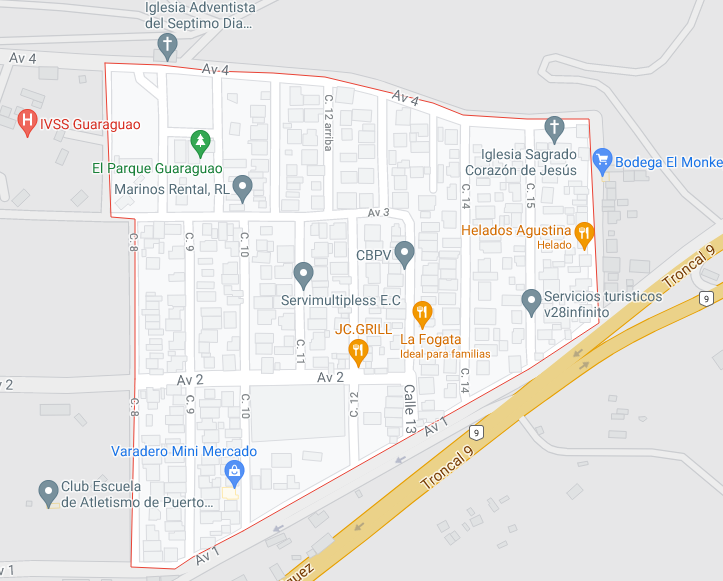
\includegraphics[width=15cm]{Media/Urb Guaraguao.png}
    \raggedright Fuente: Google Maps
    \label{fig:mapa}
\end{figure}

{\setlength{\parskip}{0cm}
\section{Nivel de Investigación}

\say{El nivel de investigación se refiere al grado de profundidad con que se aborda un fenómeno u objeto de estudio. Según el nivel, la investigación se clasifica en: Investigación Exploratoria, Investigación Descriptiva e Investigación Explicativa} (Arias, 2012).
}

En este proyecto de investigación se manifestó un nivel de investigación descriptivo. \say{La investigación descriptiva consiste en la caracterización de un hecho, fenómeno, individuo o grupo, con el fin de establecer su estructura o comportamiento.} (Arias, 2012). Se encuentra en dicho nivel, debido a que se caracterizaron las técnicas de manejo de los desechos sólidos de la población de la Urbanización Guaraguao Campo Obrero, y también, se estudiaron los beneficios de las 3R de la ecología y su aplicación en el área de estudio. 

{\setlength{\parskip}{0cm}
\section{Tipo de Investigación}

\say{El tipo de investigación es la estrategia general que adopta el investigador para responder al problema planteado. En atención al tipo, la investigación se clasifica en Investigación Documental, Investigación de Campo e Investigación Experimental.} (Arias, 2012).
}

El tipo de investigación que correspondió a este proyecto de investigación fue de campo. \say{La investigación de campo es aquella que consiste en la recolección de datos directamente de los sujetos investigados, o de la realidad donde ocurren los hechos (datos primarios).} (Arias, 2012). Es de campo porque se recolectaron los datos directamente de la población de la Urbanización Guaraguao de Puerto La Cruz, aplicando las técnicas e instrumentos propuestos para cumplir con los objetivos planteados.

{\setlength{\parskip}{0cm}
\section{Población y muestra}

\subsection{Población}

\say{La población, o en términos más precisos población objetivo, es un conjunto finito o infinito de elementos con características comunes para los cuales serán extensivas las conclusiones de la investigación. Ésta queda delimitada por el problema y por los objetivos del estudio.} (Arias, 2012). En este estudio, la población fue finita y consistió en, aproximadamente, 700 casas de la Urbanización Guaraguao de Puerto La Cruz.
}

{\setlength{\parskip}{0cm}
\subsection{Muestra}

\say{La muestra es un subconjunto representativo y finito que se extrae de la población accesible} (Arias, 2012). La muestra representativa estuvo compuesta por 22 casas pertenecientes a la calle 11 de la Urbanización Guaraguao Campo Obrero. Dicha muestra fue seleccionada mediante el muestreo intencional u opinático \say{En este caso los elementos son escogidos con base en criterios o juicios preestablecidos por el investigador.} (Arias, 2012).
}

{\setlength{\parskip}{0cm}

\section{Técnicas e Instrumentos de Recolección de Datos}

\say{Las técnicas de recolección de datos son procedimientos o fórmulas particulares de obtener datos o información}. (Arias, 2012).
}

\say{Un instrumento de recolección de datos es cualquier recurso, dispositivo o formato (en papel o digital), que se utiliza para obtener, registrar o almacenar información}. (Arias, 2012).

En este proyecto de investigación se emplearon las siguientes técnicas e instrumentos de recolección de datos:

\begin{itemize}
    \item Se utilizó la encuesta escrita como técnica de recolección de datos: “Se define a la encuesta como una técnica que pretende obtener información que suministra un grupo o muestra de sujetos acerca de sí mismos, o en relación con un tema particular. La  encuesta puede ser oral o escrita. La encuesta escrita es la que se realiza mediante un cuestionario” (Arias, 2012). Su instrumento correspondiente fue el cuestionario de preguntas cerradas: “El cuestionario es la modalidad de encuesta que se realiza de forma escrita, está formado por una serie de preguntas. El cuestionario puede ser de preguntas cerradas (cuando se establecen previamente las posibles respuestas), abiertas (cuando no ofrecen opciones de respuesta) y mixtas (cuando combina preguntas abiertas y cerradas)” (Arias, 2012). Fueron empleados con el fin de determinar los hábitos del manejo de desechos sólidos de la muestra y evaluar el conocimiento que poseían respecto a este tema a través de preguntas cerradas.
    
    \item Se usó la observación estructurada participante como técnica de recolección de datos: “La observación es una técnica que consiste en visualizar o captar mediante la vista, en forma sistemática, cualquier hecho, fenómeno o situación que se produzca en la naturaleza o en la sociedad. La observación participante es cuando el investigador pasa a formar parte de la comunidad o medio donde se desarrolla el estudio, se clasifica en observación no estructurada y observación estructurada. La observación participante estructurada es aquella que además de realizarse en correspondencia con unos objetivos, utiliza una guía diseñada previamente, en la que se especifican los elementos que serán observados” (Arias, 2012). Su instrumento correspondiente fue la lista de cotejo, “Es un instrumento en el que se indica la presencia o ausencia de un aspecto o conducta a ser observada.” (Arias, 2012), y la lista de frecuencia \say{Es un instrumento que se diseña para registrar cada vez que se presenta una conducta o comportamiento} (Arias, 2012). Fueron utilizados para la recolección de datos ya que permitían registrar de forma organizada la frecuencia con que se aplicaron las estrategias propuestas para poner en práctica las 3R de la ecología en la muestra seleccionada.
\end{itemize}

{\setlength{\parskip}{0cm}
\section{Procedimiento}

En primer lugar, se describieron los beneficios que traen consigo la aplicación de las 3R de la ecología. Para ello, se realizó una investigación documental sobre los mismos explicando el porqué es importante implementar los métodos de reciclaje, reducción y reutilización en la vida cotidiana de las personas, y los beneficios que acarrea esto para las comunidades y el medio ambiente.
}

Después, se determinaron los métodos empleados por la población para el manejo adecuado de la basura. Los habitantes del área de estudio explicaron sus hábitos para el manejo de desechos sólidos: si clasificaban una parte de los mismos, los materiales que reutilizaban para beneficio ambiental y propio, etc. 

Para ello, se aplicó una encuesta escrita de 8 preguntas cerradas a los 22 hogares que representaron a la muestra seleccionada, y así conocer su rutina en el marco del manejo de basura.

Posteriormente, se realizó una campaña divulgativa sobre el manejo adecuado de los desechos sólidos para la sensibilización del uso de las 3R de la ecología, con el fin de que los habitantes de la urbanización tengan el conocimiento necesario acerca de las 3R (reducir, reciclar y reutilizar) y cómo ponerlas en práctica. En este paso se distribuyeron folletos por cada casa en la muestra seleccionada y se dio una breve charla explicando los beneficios de las 3R de la ecología en la comunidad y cómo a través de estrategias pueden poner en práctica sus principios en el ámbito doméstico. Además, se ejecutó una segunda encuesta escrita de 6 preguntas cerradas para determinar el impacto de la campaña divulgativa en los habitantes.

Finalmente, se efectuó un seguimiento de las estrategias propuestas para el empleo de las 3R de la ecología, observando que medidas planteadas en la campaña divulgativa se lograron poner en práctica por los habitantes y con que frecuencia. Para esto, se realizó la observación participante estructurada y se rellenaron listas de cotejo por cada hogar de la muestra seleccionada. 

{\setlength{\parskip}{0cm}
\section{Técnicas de Análisis de Datos}

\say{La aplicación sistemática de técnicas estadísticas y lógicas para describir el alcance de los datos, modular la estructura de los datos, condensar la representación de los datos, ilustrarlos mediante imágenes, tablas y gráficos, y evaluar las inclinaciones estadísticas, los datos de probabilidad, para obtener conclusiones significativas, se conoce como análisis de datos.} (Arteaga, 2020). Pueden provenir de varias fuentes y pueden tener formato de texto, de audio, de imagen o de vídeo.
}

Para analizar los resultados cuantitativos, se utilizaron las siguientes técnicas de análisis:

\begin{itemize}
    \item Gráfico de barras: \say{Un gráfico de barras es una forma de resumir un conjunto de datos por categorías. Muestra los datos usando varias barras de la misma anchura, cada una de las cuales representa una categoría concreta.} (TIBCO, 2014). Se empleó el gráfico de barras porque permitía comparar gráficamente cuales indicadores de las tablas presentaron mayor frecuencia en la población de estudio.

    \item Tabla: \say{En computación, una tabla hace referencia al modelado o recopilación de datos por parte de una aplicación de un programa que permite operar con los mismos organizándolos y poniéndolos en relación de diversas maneras. Son estructuras útiles y a menudo fáciles de interpretar para relacionar datos e información de manera pertinente.} (Bembibre, 2009). Se usó la tabla para poder recopilar de manera organizada los resultados cuantitativos que fueron obtenidos.
\end{itemize}

\newpage

\section{Cronograma} 

\begin{figure}[h]
    \centering
    \captionsetup{singlelinecheck=false, justification=raggedright, labelsep=newline}
    \caption{\textit{Cronograma de actividades detalladas en los objetivos del proyecto}}
    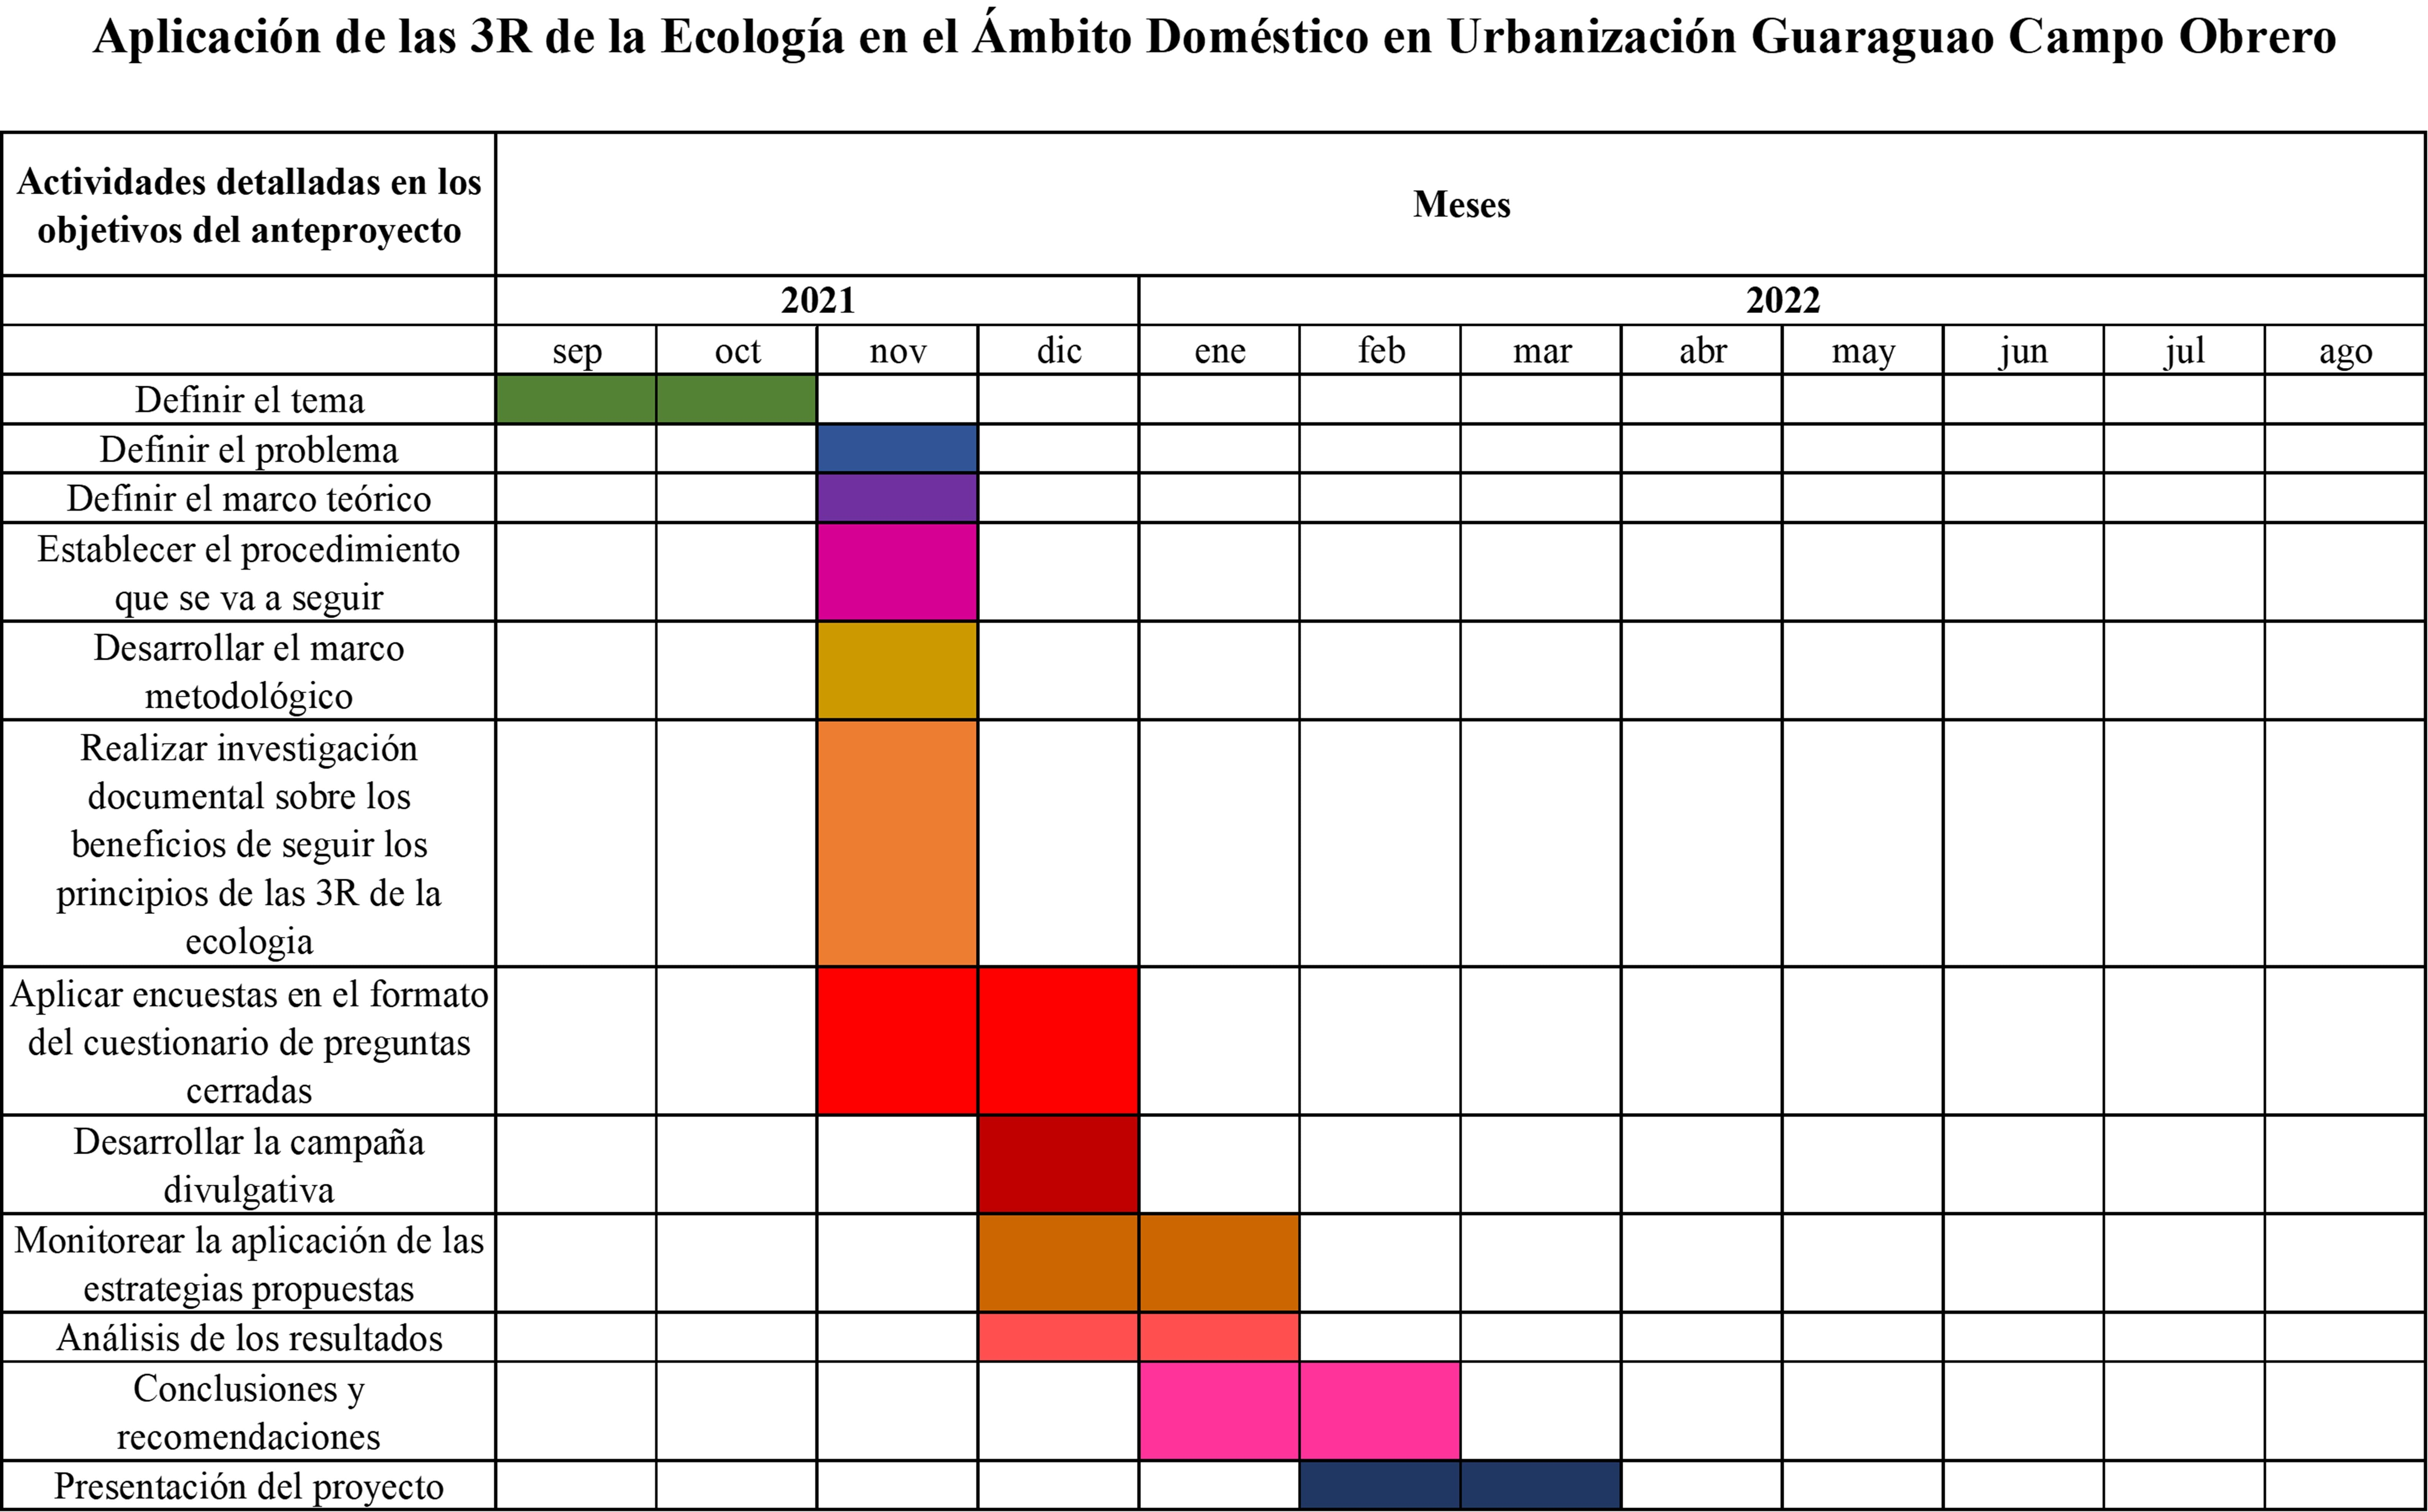
\includegraphics[width=15cm]{Media/Cronograma.jpg}
    \raggedright Fuente: Elaboración propia
    \label{fig:cronograma}
\end{figure}

\newpage % colocar página del capítulo 3
    \vspace*{6cm}
\chapter{Resultados y discusión}
\newpage
 % colocar página del capítulo 4
    \vspace*{6cm}
{\setlength{\parskip}{-0.5cm}
\chapter{Conclusiones y recomendaciones}
}
\newpage

En este capítulo se concluyen los resultados obtenidos del trabajo y se dan recomendaciones para futuras investigaciones.

{\setlength{\parskip}{0cm}
\section{Conclusiones}

\begin{itemize}
    \item Se concluyó que las 3R de la ecología son necesarias para la defensa del medio ambiente, y que la disminución de la emisión de gases de efecto invernadero y de residuos sólidos, el ahorro de la energía, la reducción de la deforestación, entre otros, son algunos de los grandes beneficios de estos principios al medio ambiente.
    
    \item Se evidenció que la mayoría de la población no ponía en práctica o desconocía algunas de las estrategias de las 3R de la ecología. Sin embargo, las personas que conformaron la muestra seleccionada estuvieron de acuerdo en que su rutina del manejo de desechos sólidos podía mejorarse para minimizar los daños colaterales por la generación de los mismos. También mostraron tener algunos hábitos con respecto a la reutilización del plástico, vidrio, cartón, papel y desechos orgánicos. 
    
    \item Se logró captar la atención de la muestra a través de la campaña divulgativa. También su interés en contribuir en la iniciativa de aplicar estrategias propuestas acerca de estos principios del desarrollo sustentable. En este sentido, se observó un cambio positivo en sus hábitos de manejo de los desechos sólidos.
    
    \item Se observó, mediante el seguimiento realizado, que algunas de las estrategias propuestas para el empleo de las 3R de la ecología fueron implementadas con mayor facilidad por la muestra, como reutilizar frascos para almacenar objetos y evitar el uso de platos, cucharas y vasos desechables. Por el contrario, hubo otras que fueron poco aplicadas como, usar botellas plásticas como macetas para plantas y evitar comprar artículos empaquetados con exceso de plástico.
\end{itemize}
}

\newpage

{\setlength{\parskip}{0cm}
\section{Recomendaciones}

\begin{itemize}
    \item Extender la información acerca de los beneficios sobre la aplicación de las estrategias planteadas en la campaña divulgativa para el empleo de las 3R de la ecología a todo el conjunto residencial. 
    
    \item Hacer el seguimiento de la implementación de las estrategias propuestas con mayor frecuencia.

    \item Aplicar las estrategias propuestas en todo el conjunto residencial.
    
    \item Formar brigadas ecológicas en el sector a fin de que sean estas las que promuevan la aplicación de las 3R en el área de estudio.
\end{itemize}
}

\newpage % colocar página del capítulo 1
    \nocite{*}
    {\setlength{\parskip}{-0.5cm}
    \printbibliography
    }
    \newpage

{\setlength{\parskip}{0cm} {
\chapter*{Anexos}

\setlength{\parindent}{0ex}

\textbf{Anexo 1} \\
\textit{Modelo de la encuesta distribuida para el establecimiento de los métodos empleados por la población en la Urbanización Guaraguao de Puerto La Cruz}
}

\begin{figure}[!ht]
    \centering
    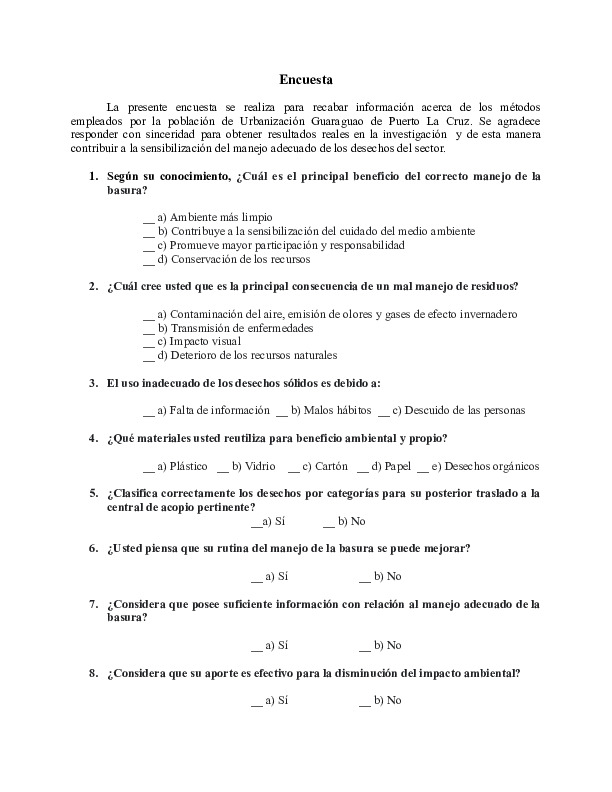
\includegraphics[width=13cm]{Media/Encuesta 1.jpg}
    \label{fig:encuesta}
\end{figure}

\setlength{\parindent}{0ex}

Fuente: Elaboración propia

\newpage

\setlength{\parindent}{0ex}

\textbf{Anexo 2} \\
\textit{Folleto entregado durante la campaña divulgativa realizada en la Urbanización Guaraguao de Puerto La Cruz}
}
\begin{figure}[!ht]
    \centering
    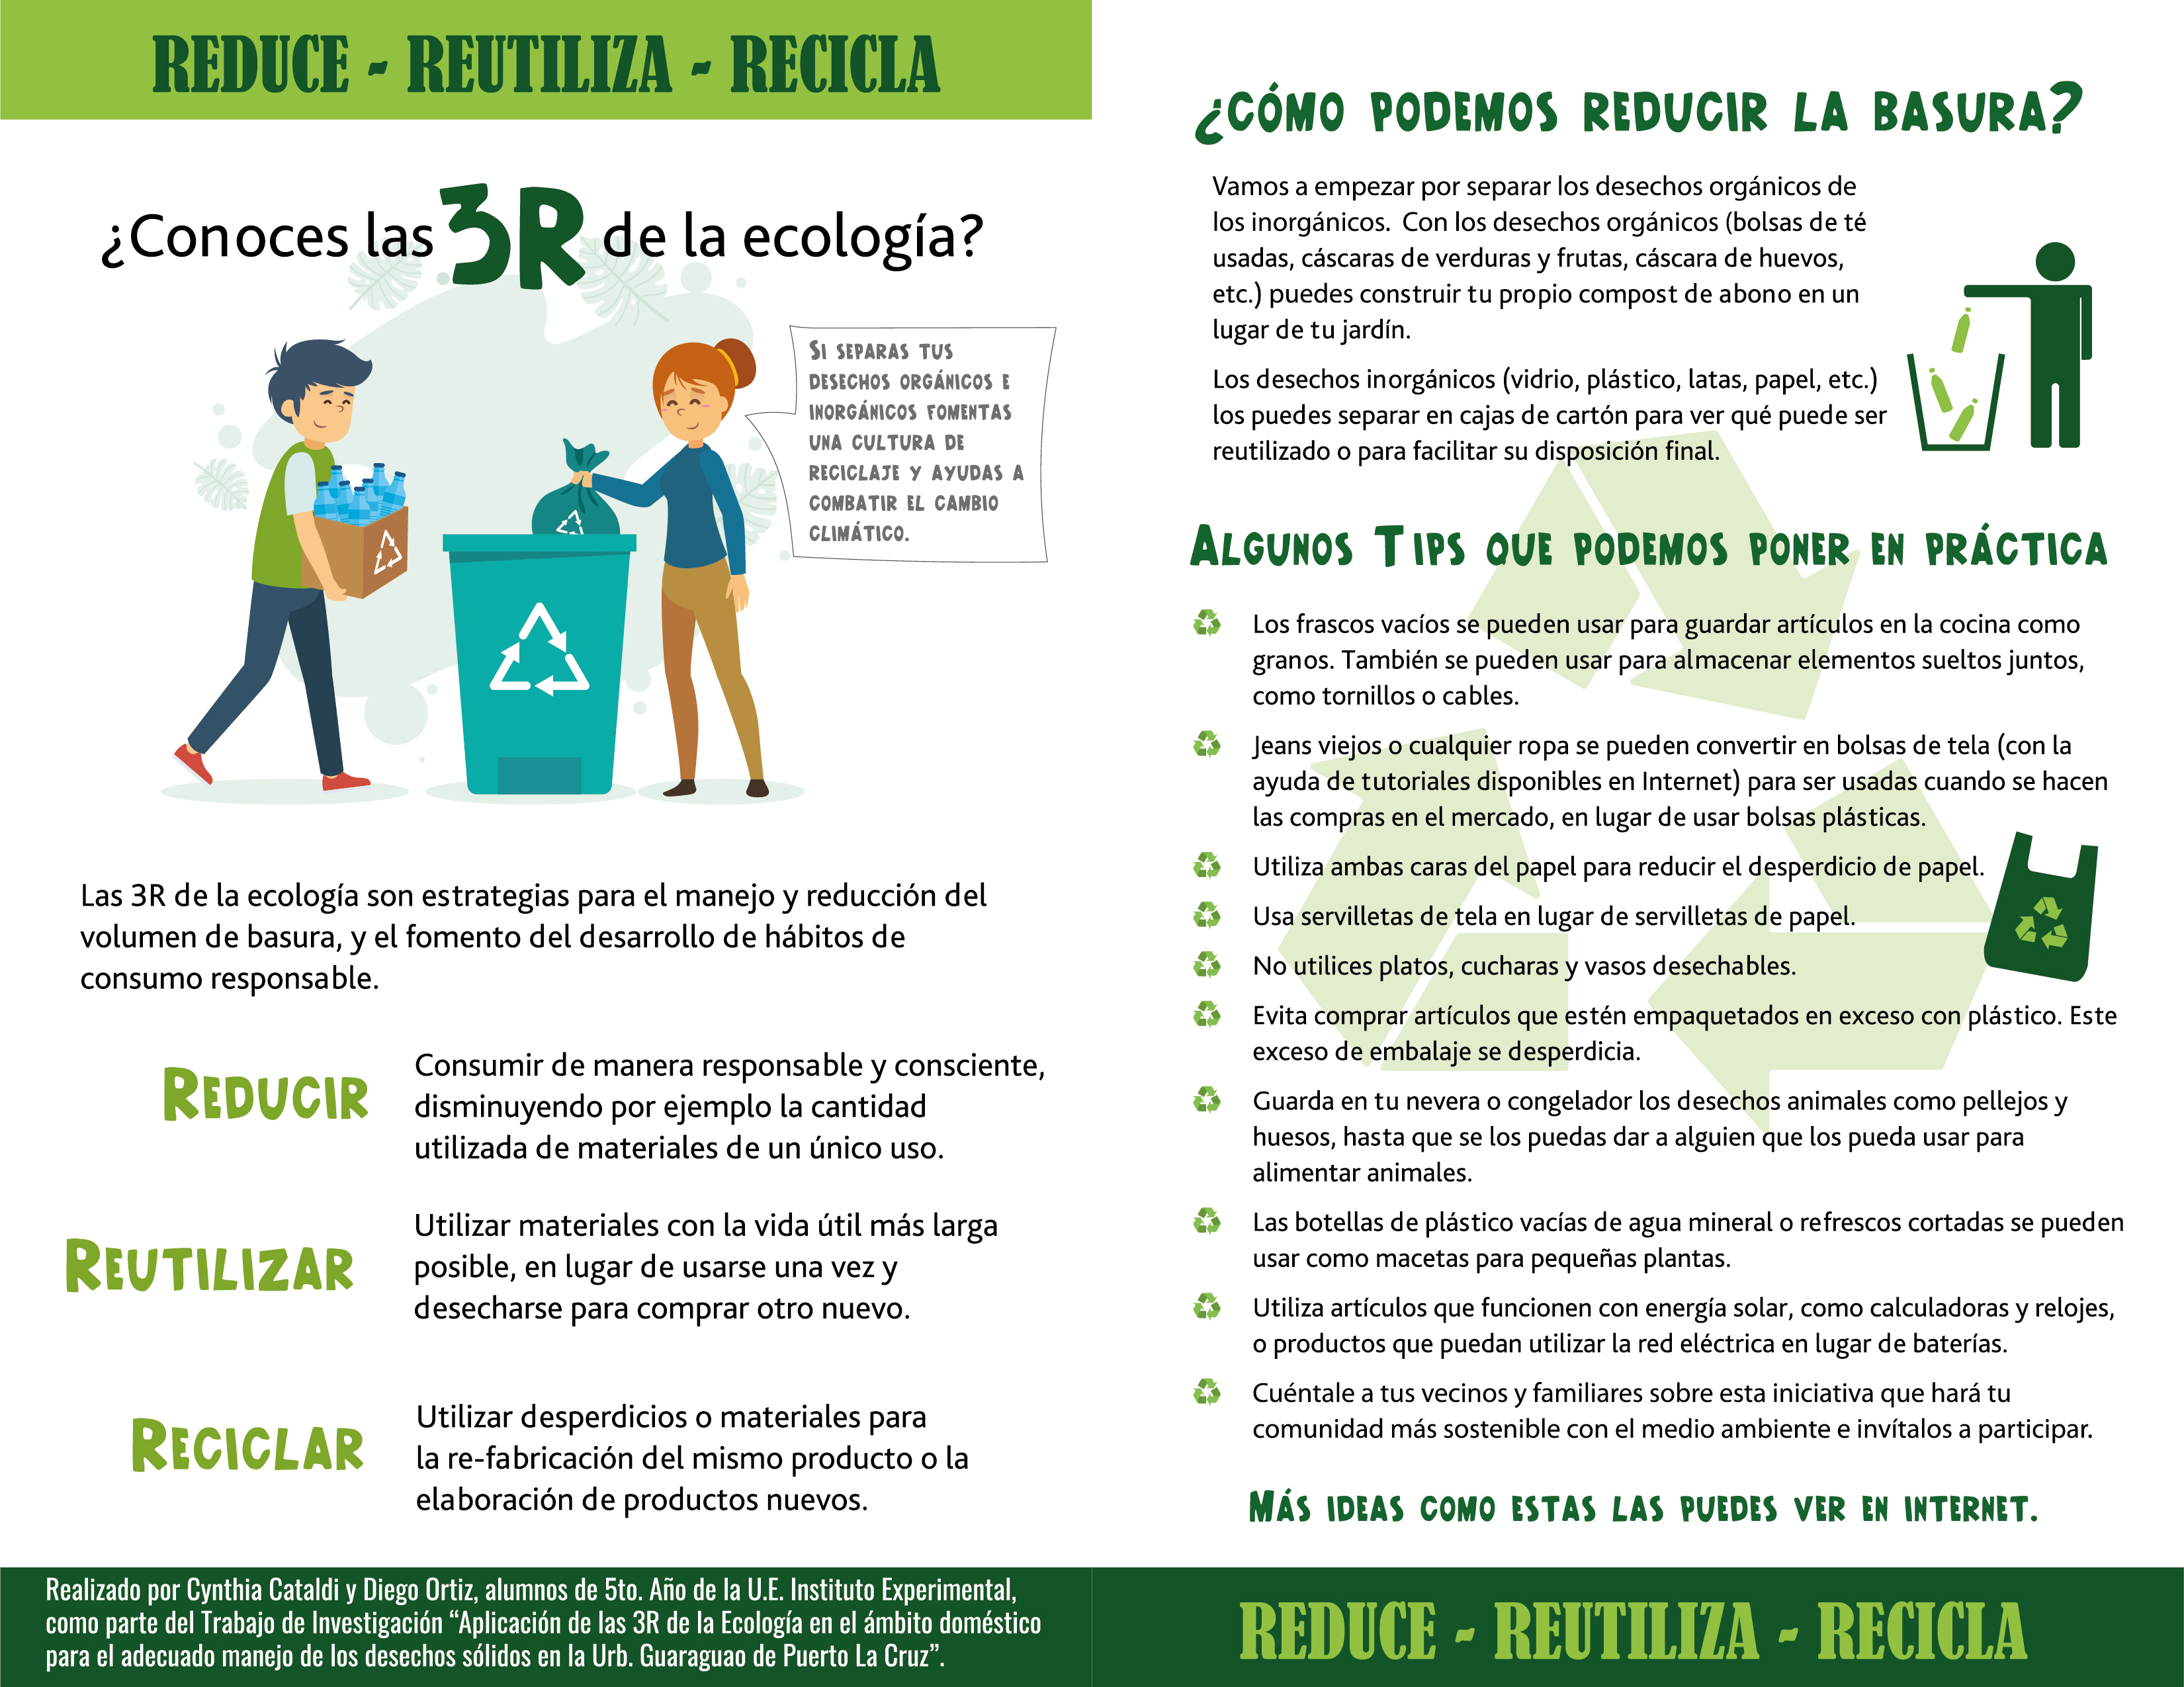
\includegraphics[width=17cm, angle=90]{Media/Volante.jpg}
    \label{fig:folleto}
\end{figure}

\setlength{\parindent}{0ex}

Fuente: Elaboración propia

\newpage

\setlength{\parindent}{0ex}

\textbf{Anexo 3} \\
\textit{Modelo de la encuesta distribuida para determinar los cambios en los hábitos del manejo de la basura a raíz de la campaña divulgativa realizada en la Urbanización Guaraguao de Puerto La Cruz}

\begin{figure}[!ht]
    \centering
    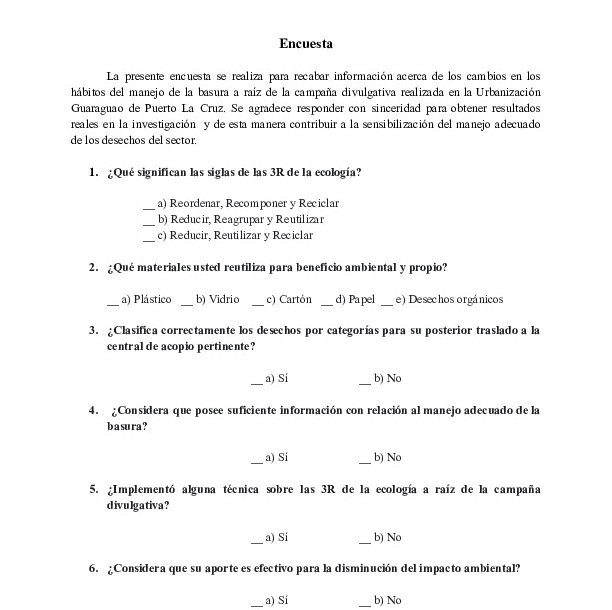
\includegraphics[width=15cm]{Media/Encuesta 2.jpg}
    \label{fig:encuesta2}
\end{figure}

\setlength{\parindent}{0ex}

Fuente: Elaboración propia

\newpage

\textbf{Anexo 4} \\
\textit{Lista de Cotejo realizada para el seguimiento de las estrategias propuestas para la aplicación de las 3R de la ecología en la Urbanización Guaraguao de Puerto La Cruz}

\begin{figure}[!ht]
    \centering
    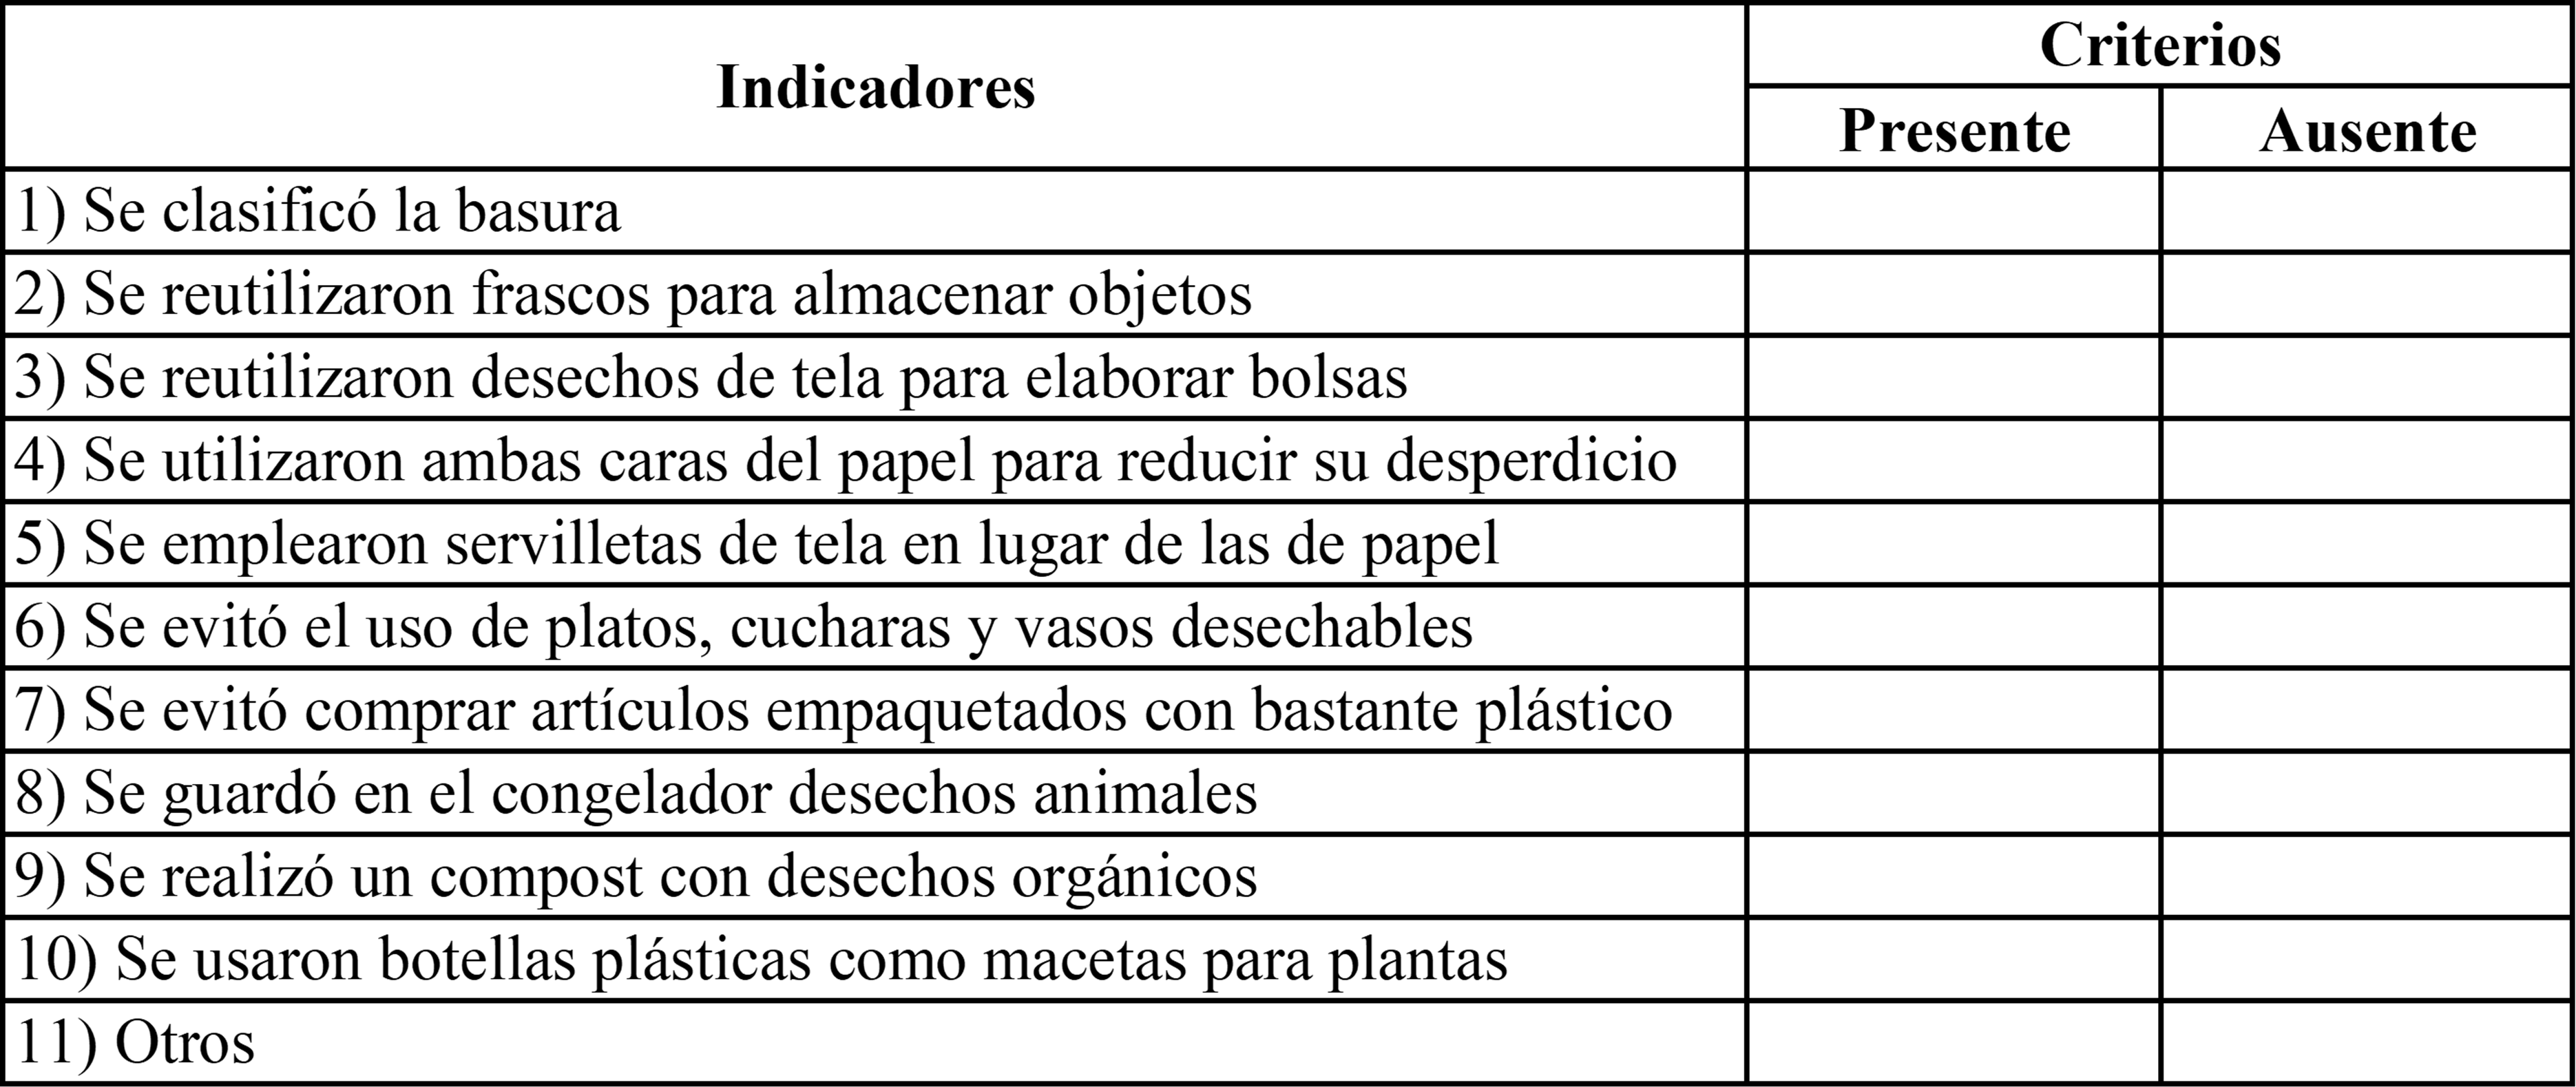
\includegraphics[width=15cm]{Media/lista de cotejo.png}
    \label{fig:ListadeCotejo}
\end{figure}

\setlength{\parindent}{0ex}

Fuente: Elaboración propia

\newpage

\textbf{Anexo 5} \\
\textit{Otras estrategias aplicadas por la muestra seleccionada para la aplicación de las 3R de la ecología}

\begin{figure}[!ht]
    \centering
    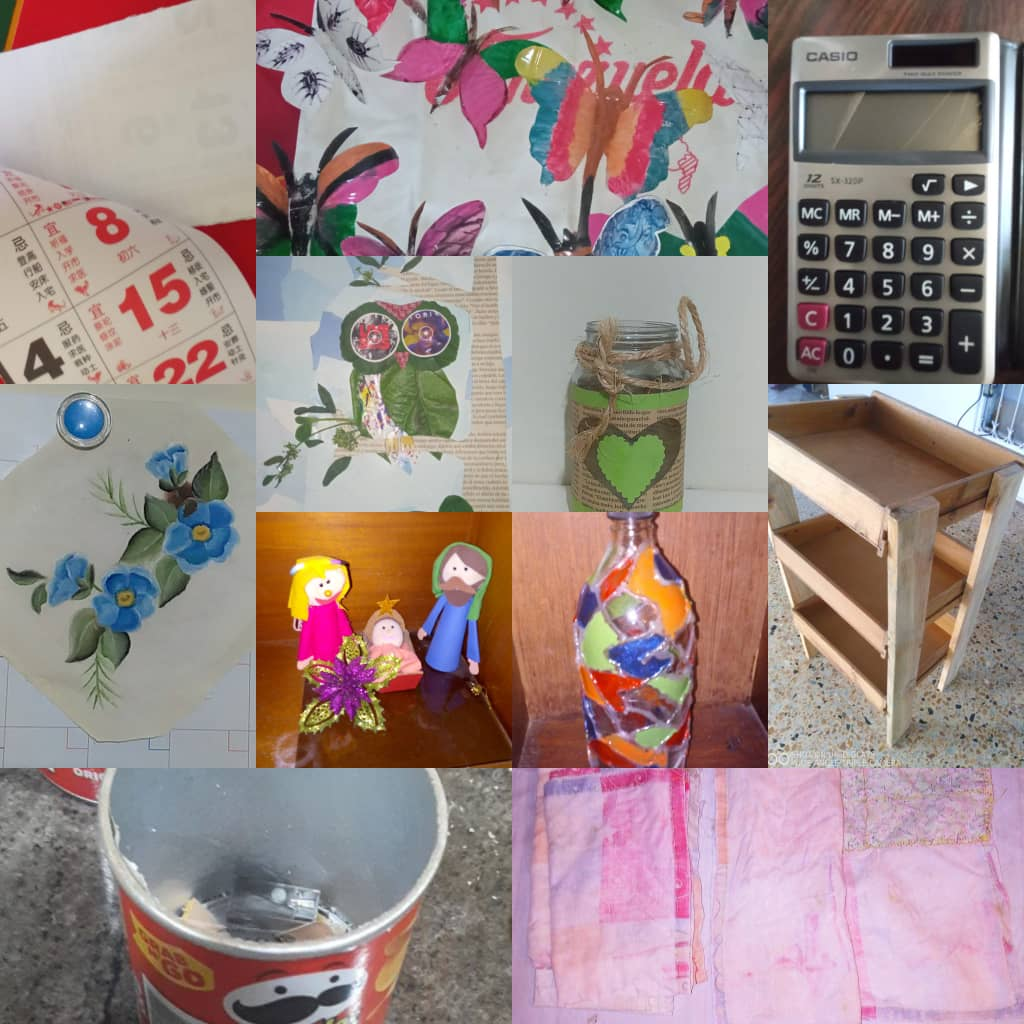
\includegraphics[width=15cm]{Media/Fotos/Foto 1 otros.jpeg}
    \label{fig:anexo5}
\end{figure}

\setlength{\parindent}{0ex}

Fuente: Elaboración propia

\newpage

\textbf{Anexo 6} \\
\textit{Estrategia de almacenar desechos animales en el congelador}

\begin{figure}[!ht]
    \centering
    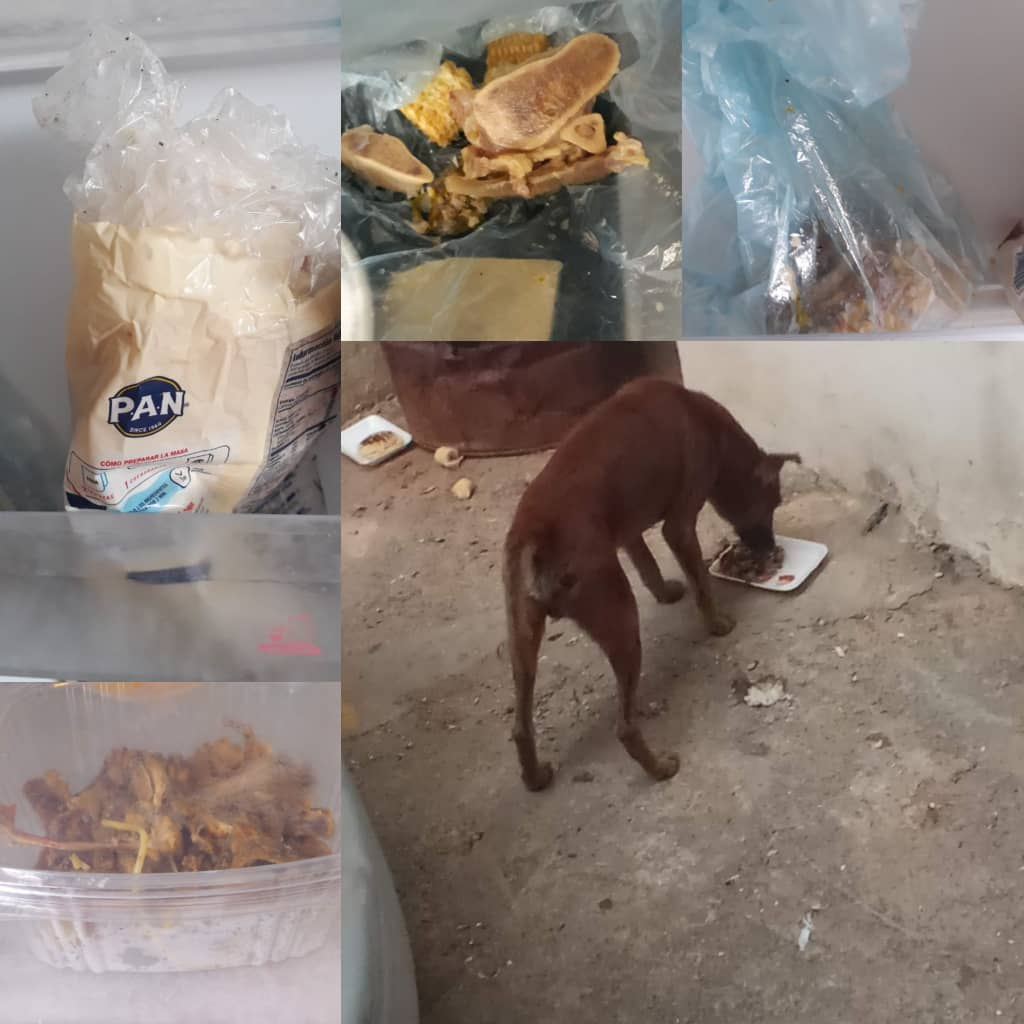
\includegraphics[width=15cm]{Media/Fotos/Foto 2 huesos.jpeg}
    \label{fig:anexo6}
\end{figure}

\setlength{\parindent}{0ex}

Fuente: Elaboración propia

\newpage

\textbf{Anexo 7} \\
\textit{Reutilización de envases para almacenar objetos}

\begin{figure}[!ht]
    \centering
    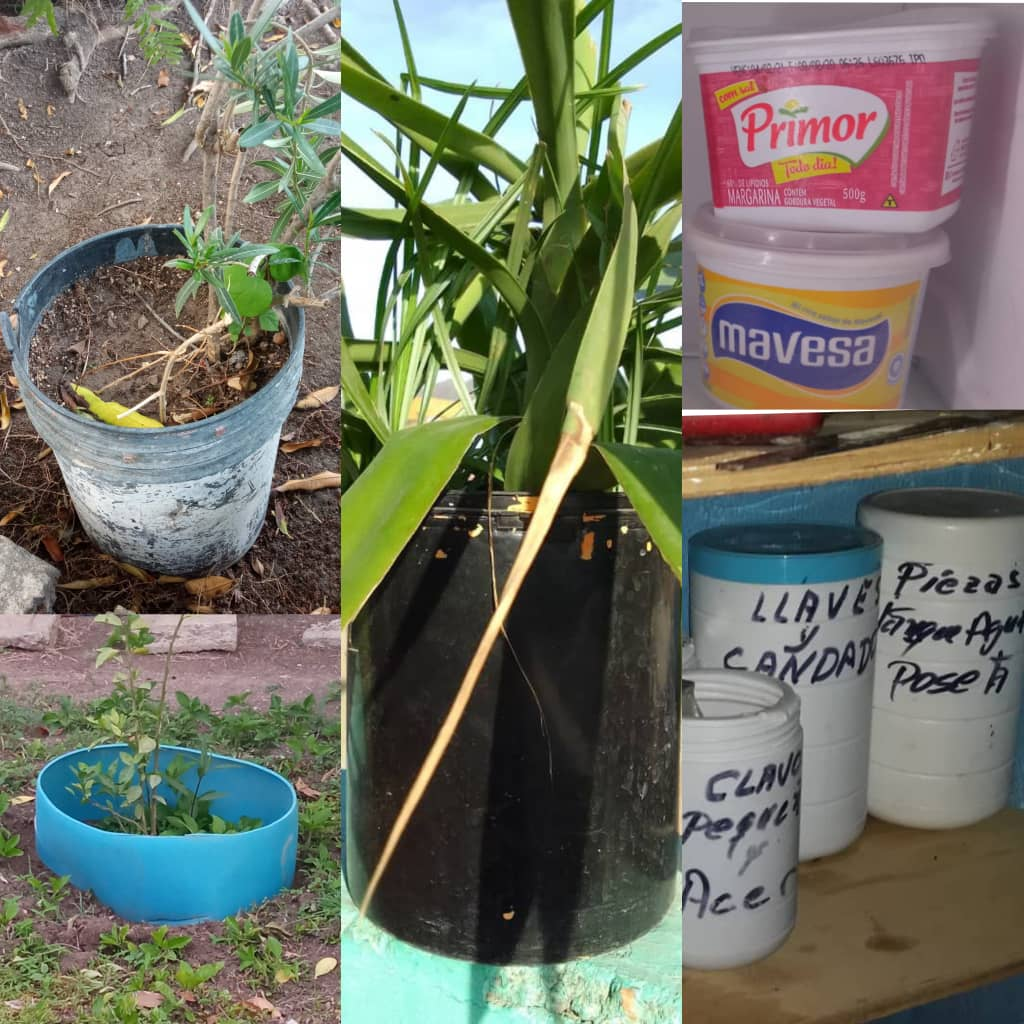
\includegraphics[width=15cm]{Media/Fotos/Foto 3 envases.jpeg}
    \label{fig:anexo7}
\end{figure}

\setlength{\parindent}{0ex}

Fuente: Elaboración propia

\newpage

\textbf{Anexo 8} \\
\textit{Reutilización de frascos para almacenar objetos}

\begin{figure}[!ht]
    \centering
    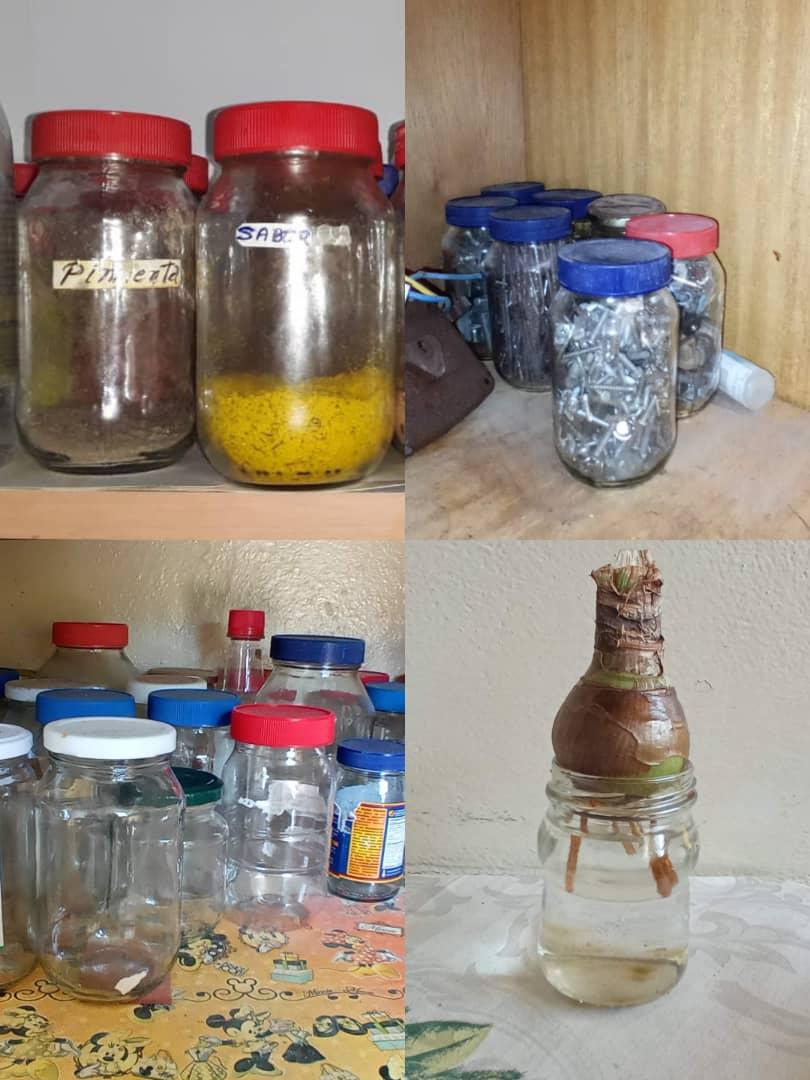
\includegraphics[width=15cm]{Media/Fotos/Foto 4 Frascos.jpeg}
    \label{fig:anexo9}
\end{figure}

\setlength{\parindent}{0ex}

Fuente: Elaboración propia

\newpage

\textbf{Anexo 9} \\
\textit{Elaboración de compost con desechos orgánicos}

\begin{figure}[!ht]
    \centering
    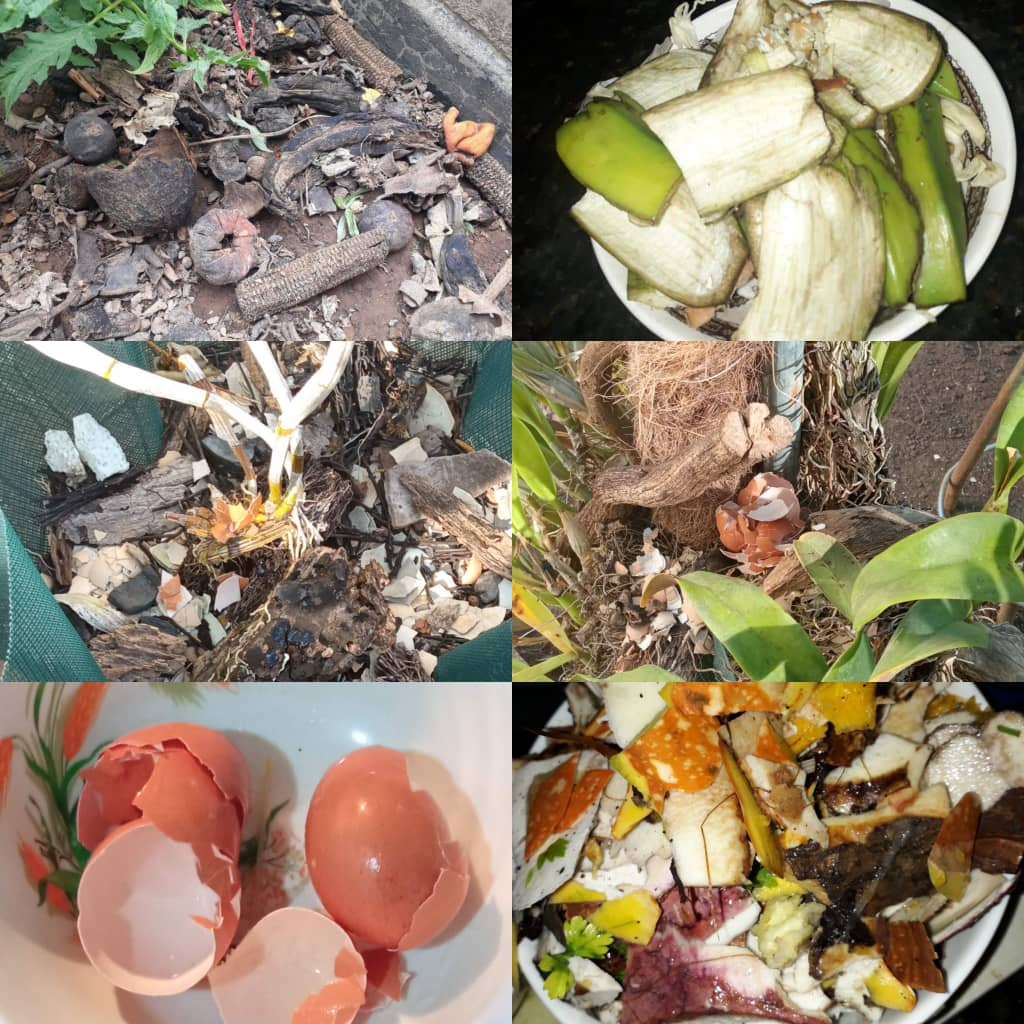
\includegraphics[width=15cm]{Media/Fotos/Foto 5 Compost.jpeg}
    \label{fig:anexo10}
\end{figure}

\setlength{\parindent}{0ex}

Fuente: Elaboración propia

\newpage

\textbf{Anexo 10} \\
\textit{Reutilización de hojas de papel}

\begin{figure}[!ht]
    \centering
    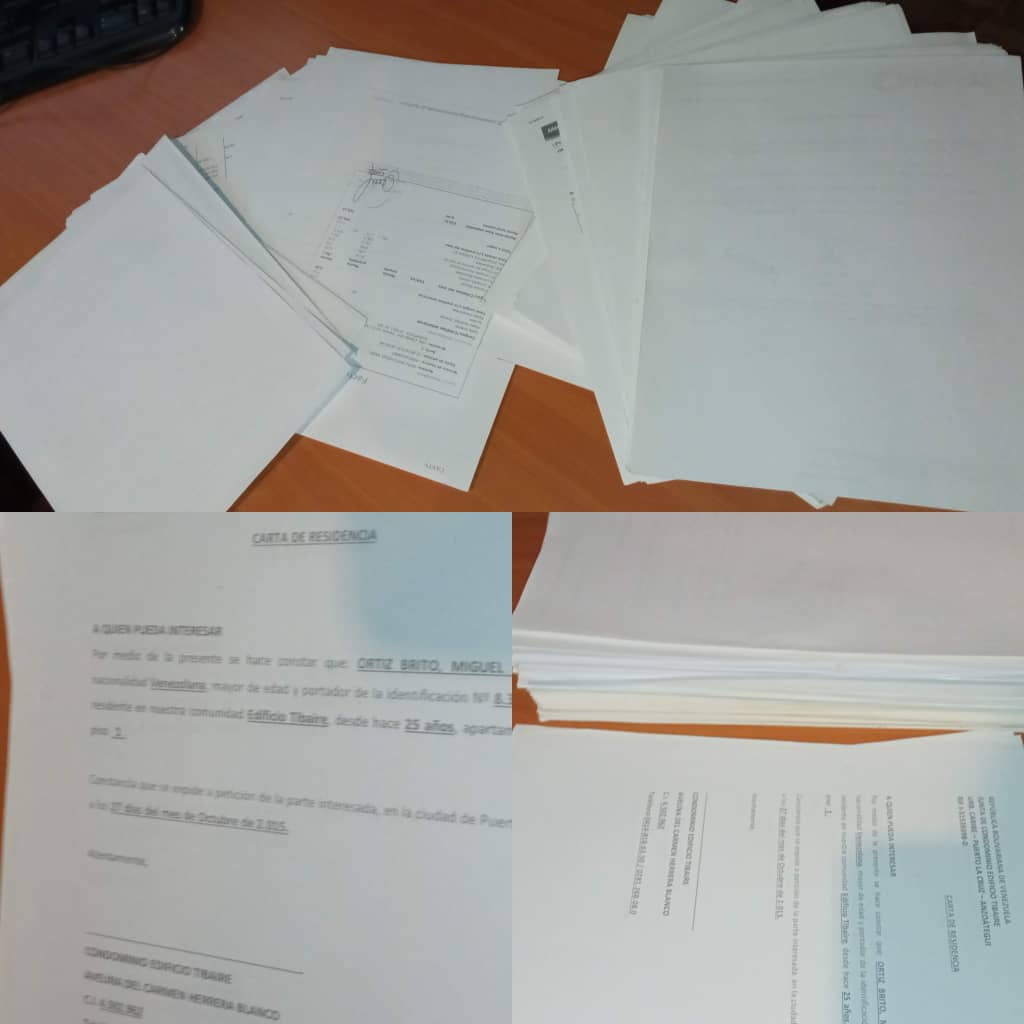
\includegraphics[width=15cm]{Media/Fotos/Foto 8 papel.jpeg}
    \label{fig:anexo11}
\end{figure}

\setlength{\parindent}{0ex}

Fuente: Elaboración propia

\newpage

\textbf{Anexo 11} \\
\textit{Clasificación casera de los desechos sólidos}

\begin{figure}[!ht]
    \centering
    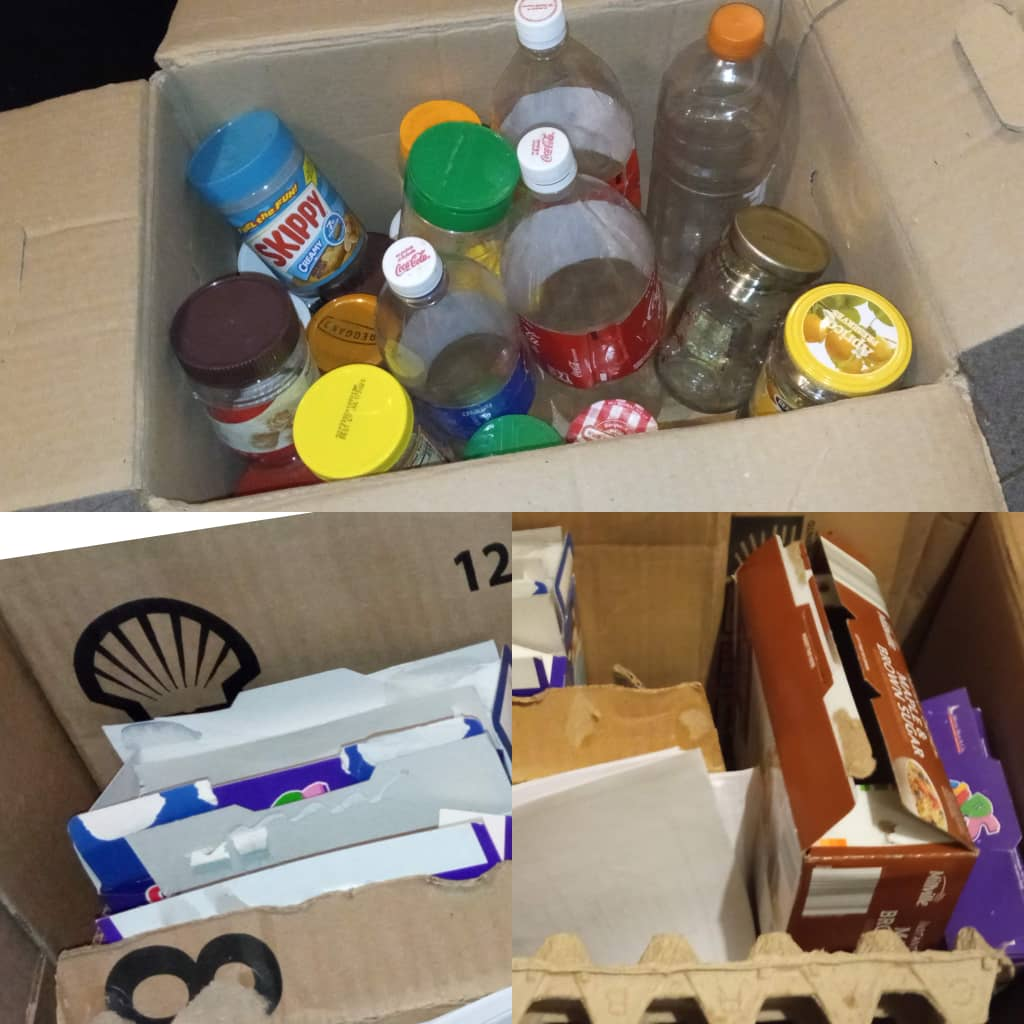
\includegraphics[width=15cm]{Media/Fotos/Foto final clasificacion.jpeg}
    \label{fig:anexo12}
\end{figure}

\setlength{\parindent}{0ex}

Fuente: Elaboración propia
 % colocar página de anexos
\end{document}
% final del documento ;D